%\pagestyle{art}
\chapter[Artes visuais, dança, música e teatro]{\LARGE Artes visuais, dança, música e teatro}
\markboth{Módulo 1}{}

\vspace*{-1cm}
\enlargethispage{2\baselineskip}

\section*{Habilidades do SAEB}

\begin{itemize}
\item Reconhecer elementos constitutivos das artes visuais, dança, música e
teatro.

\item Identificar formas distintas de artes visuais em diferentes suportes e
mídias.

\item Identificar características do sistema de circulação das artes
visuais, dança, música e teatro em diferentes contextos (teatros,
palcos, museus, galerias, artistas, artesãos, curadores, produtores
etc.).

\item Identificar distintas formas e/ou gêneros de expressão da dança, da
música e do teatro em diferentes contextos e práticas.
\end{itemize}

\subsection{Habilidades da BNCC}

\begin{itemize}
\item EF15AR01, EF15AR02, EF15AR08, EF15AR13, EF15AR14, EF15AR18.
\end{itemize}


\conteudo{Na língua portuguesa, existem as linguagens verbais e
não verbais. Na linguagem verbal, a comunicação ocorre por meio da palavra (oral ou
escrita). Na linguagem não verbal, a comunicação acontece, por exemplo, por meio de
expressões faciais, mímicas, desenhos, coreografias ou semáforos.

A linguagem é uma atividade humana e pode se manifestar de diversos
modos, dependendo da intenção no momento da
comunicação. Para que você possa se comunicar bem, precisa ter
experiências com variadas formas de comunicação.

Na arte, assim como na língua, a linguagem artística, também
compreendida como atividade humana, manifesta-se de diferentes modos,
por meio de materialidades verbais e não verbais, sempre relacionadas à
história, à cultura e à sociedade de cada grupo. Para que suas
experiências com a arte e suas linguagens sejam enriquecidas, é preciso
ampliar suas práticas artísticas de apreciação, análise, reflexão e
criação.

\begin{itemize}
\item
  \textbf{Artes visuais}
\end{itemize}

São exemplos de artes visuais, ou seja, manifestações artísticas que têm
a expressão relacionada ao sentido da visão: arquitetura, artesanato,
cinema, desenho, escultura, fotografia e pintura.

\pagebreak
\begin{itemize}
\item
  \textbf{Dança}
\end{itemize}

São exemplos de danças, manifestações artísticas que têm o corpo como
instrumento de expressão: balé, dança do ventre, forró, frevo, maracatu,
samba e quadrilha.

\begin{itemize}
\item
  \textbf{Música}
\end{itemize}

São exemplos de músicas, manifestações artísticas que têm o som como
meio de expressão: axé, eletrônica, forró, funk, gospel, hip-hop e
samba.

\begin{itemize}
\item
  \textbf{Teatro}
\end{itemize}

Já no teatro, o fazer teatral se dá principalmente pela
reunião de três elementos básicos: o(s) ator(es), o texto e o público.}

% \coment{Sugerimos que a primeira leitura do texto seja realizada pelos alunos
% individualmente. Depois, faça uma roda de conversa e oriente a discussão
% coletiva sobre o texto, fazendo perguntas, como estas:
% Como o texto comparou nossa língua e a arte? Essa comparação auxiliou na
% compreensão sobre a importância das linguagens artísticas no seu dia a
% dia? O que você entendeu por artes plásticas? Quais são as manifestações
% das artes plásticas citadas no texto? Quais outras manifestações das
% artes plásticas você conhece que não foram citadas no texto? Na
% dança, quais manifestações foram citadas pelo texto? Você conhece
% outras manifestações de dança? Na música, quais manifestações foram
% citadas? Você conhece outras manifestações de música? Quais são os
% elementos básicos do teatro?}

\section*{Atividades}

\num{1} Você pode utilizar várias partes do seu corpo para produzir sons.
Bata palmas tendo como base as ilustrações de cada tipo de palma e
prestando atenção nos sons que elas produzem: graves ou agudos.

\begin{figure}[htpb!]
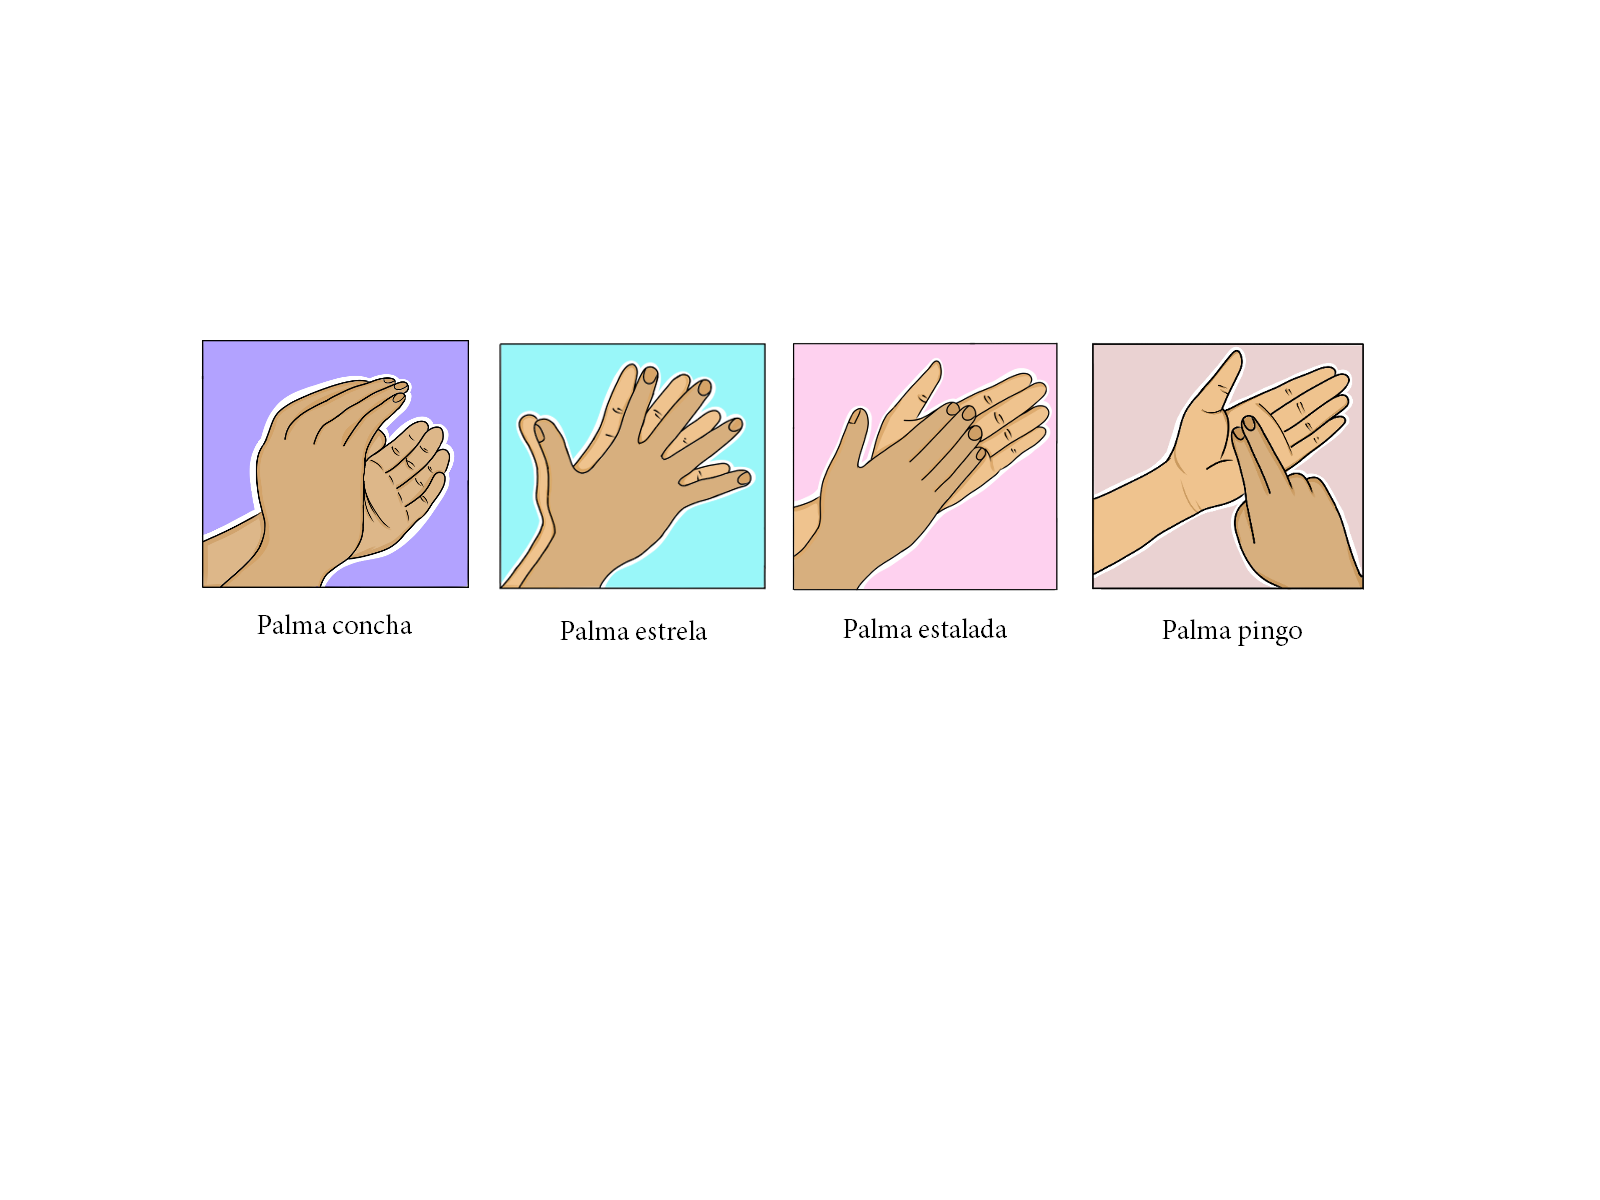
\includegraphics[width=\textwidth]{../ilustracoes/ART5/SAEB_5ANO_ART_FIGURA1.png}
\end{figure}

\noindent{}Agora, numere as palmas da mais grave para a mais aguda. A número 1
corresponderá à palma que produz o som mais grave, e a número 4 corresponderá à que
produz o som mais agudo.\bigskip

\begin{minipage}{.5\textwidth}
\begin{boxlist}
\boxitem{2} Palma estrela.

\boxitem{4} Palma pingo.

\boxitem{3} Palma estalada.

\boxitem{1} Palma concha.
\end{boxlist}
\end{minipage}
\sidetext{A palma concha produz o som mais grave. A palma estrela também produz um
som grave, no entanto menos grave que a palma concha. A palma estalada
produz um som agudo. E o som mais agudo, entre esses tipos de palma, é
produzido pela palma pingo.}

\num{2}  Leia o texto.

\begin{myquote}
O carimbó é um ritmo amazônico, típico do Pará, que nasceu das mãos
calejadas e dos pés descalços dos agricultores paraenses. Um ritmo, uma
dança, uma identidade. O nome carimbó ou curimbó vem do tupi:
\emph{curi} é pau oco e \emph{m'bó} é furado.

A união das palavras também batizou o tambor grande e o curimbó se toca
com as pernas abraçando o instrumento. O milheiro e as maracás completam
a sonoridade indígena. A dança de passos miúdos, em roda, também vem da
tradição dos índios, mas não seria de todo Brasil se não tivesse
mistura.

No rebolado está a herança do sangue negro, presente ainda no batuque
acelerado e no som do banjo. Do branco europeu vem o saxofone, a flauta
ou o clarinete. O jeito de dançar em rodopios, com a formação de casais,
é bem português.
{[}\ldots{}{]}

\fonte{Priscila Brandão. G1. Conheça a história do carimbó. Disponível em:
\emph{https://g1.globo.com/economia/agronegocios/noticia/2015/12/conheca-historia-do-carimbo.html}. Acesso em: 17 mar. 2023.}
\end{myquote}

\noindent{}Retire informações do texto para completar o esquema.

\begin{figure}[htpb!]
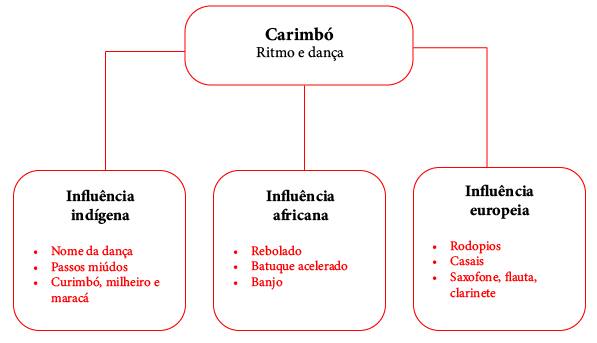
\includegraphics[width=\textwidth]{../ilustracoes/ART5/SAEB_5ANO_ART_FIGURA3.png}
\end{figure}

% \coment{Para que os alunos possam experimentar os movimentos do carimbó e
% ampliar o repertório corporal, indicamos a projeção de vídeos. Entre os
% muitos vídeos presentes na internet, sugerimos dois: \emph{Carimbó – Grupo Sarandeiros – Dançando na EEFFTO}, disponível em: \emph{https://www.youtube.com/watch?v=mqKD4kM8fHk}
% (acesso em: 19 mar. 2023); \emph{Dança do Carimbó Passos básicos Oficina de Dança e Apresentação Cultural}, disponível em: \emph{https://www.youtube.com/watch?v=-0QGO8ua2WE}
% (acesso em: 19 mar. 2023).}

\bigskip

\noindent{}Para responder às atividades 3 e 4, leia os conceitos sobre volume
bidimensional e tridimensional.

\begin{mdframed}[linewidth=2pt,linecolor=salmao,backgroundcolor=salmao!20]
\vspace{1cm}
\textbf{Bidimensional:} o que tem duas dimensões – comprimento e largura.

\vspace{1cm}

\noindent\textbf{Tridimensional:} o que apresenta três dimensões – comprimento, largura e profundidade.
\vspace{1cm}
\end{mdframed}

\num{3} Nas formas de expressão das artes a seguir, assinale B para volume bidimensional ou T para volume tridimensional.

\begin{center}
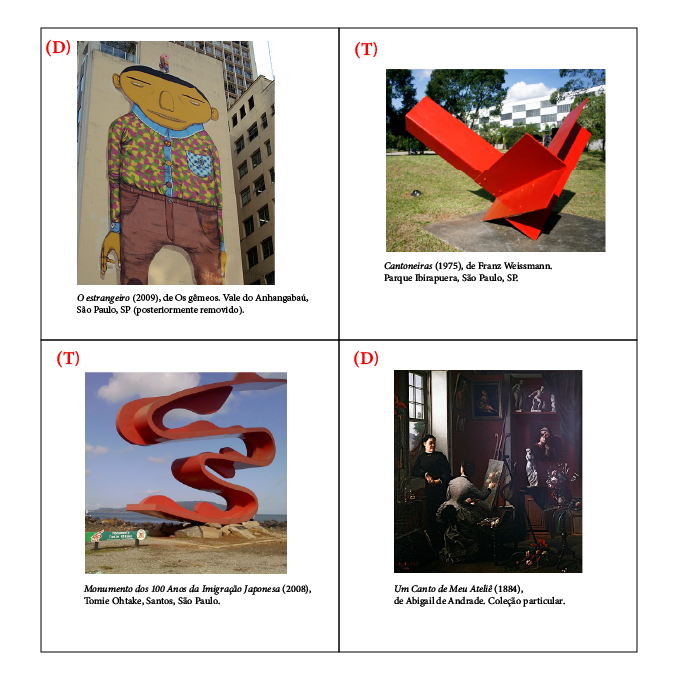
\includegraphics[width=.95\textwidth]{../ilustracoes/ART5/SAEB_5ANO_ART_FIGURA4.png}
\end{center}

\pagebreak

\conteudo{\textbf{Os Gêmeos}, como o próprio nome sugere, são uma dupla de irmãos gêmeos
grafiteiros: Gustavo e Otávio Pandolfo, nascidos em 1974, em São Paulo.
Seus trabalhos fazem parte, principalmente, do cenário paulistano, mas
também estão presentes nos Estados Unidos, na Alemanha,
na Inglaterra e, entre outros países, em Cuba.

\textbf{Franz Weissman}, escultor, desenhista, pintor e professor, nasceu em
Knittelfeld, na Áustria, em 1911. Em 1921, ainda criança, veio morar com
sua família no Brasil. Sua obra tem como base a valorização das formas
geométricas e dos espaços vazados. Foi um dos precursores do movimento
construtivismo no Brasil e criou várias esculturas em espaços públicos.

\textbf{Abigail de Andrade}, pintora e desenhista brasileira, nasceu em 1864, na
cidade de Vassouras (RJ). Ela pintava paisagens, cenas do
cotidiano carioca, retratos, autorretratos e naturezas-mortas. Foi a
primeira mulher a receber uma premiação na Exposição Geral de Belas
Artes, em 1884. No Brasil, naquela época, as mulheres tinham pouco
espaço na aprendizagem artística e eram impedidas de frequentar
oficialmente cursos na Academia Imperial de Belas Artes. Essa
participação só foi possível a partir de 1892.

\textbf{Tomie Ohtake}, pintora, gravurista e escultora, nasceu em Kyoto, no Japão,
em 1913 e chegou ao Brasil em 1936. É uma artista japonesa naturalizada
brasileira e uma das principais representantes do abstracionismo
informal, que busca inspiração no inconsciente e na intuição para
construir arte.
}

\num{4}  Dimensão é o espaço que um elemento ocupa. Associe os espaços
  dimensional e tridimensional a suas características.

\begin{multicols}{2}
1. Espaço dimensional.

2. Espaço tridimensional.

\columnbreak

\noindent{}(\rosa{1}) Apresenta figuras dispostas em superfície plana.

\noindent{}(\rosa{1}) Para criar a ilusão de profundidade, utiliza elementos como cores, linhas, textura.

\noindent{}(\rosa{2}) Os elementos são percebidos por meio de três dimensões: altura, profundidade e largura.

\noindent{}(\rosa{2}) Possui relevo, o que contribui para a percepção de texturas, dimensões e espaço.
\end{multicols}

\pagebreak

\noindent{}Para responder às atividades 5 e 6, leia o texto.

\begin{myquote}
A definição de museu passou por uma significativa mudança. A aprovação
da nova definição de museu se deu durante a 26ª Conferência Geral do
Conselho Internacional de Museus (Icom), em agosto de 2022.


A \textbf{antiga} definição estabelecia:

\emph{O museu é uma instituição permanente sem fins lucrativos, ao
serviço da sociedade e do seu desenvolvimento, aberta ao público, que
adquire, conserva, investiga, comunica e expõe o patrimônio material e
imaterial da humanidade e do seu meio envolvente com fins de educação,
estudo e deleite.}


A \textbf{nova} definição estabelece:

\emph{Um museu é uma instituição permanente, sem fins lucrativos, a
serviço da sociedade, que pesquisa, coleciona, conserva, interpreta e
expõe patrimônio material e imaterial. Abertos ao público, acessíveis e
inclusivos, os museus promovem a diversidade e a sustentabilidade. Atuam
e se comunicam de forma ética, profissional e com a participação das
comunidades, oferecendo experiências variadas de educação,
entretenimento, reflexão e compartilhamento de conhecimento.}

\fonte{Fonte de pesquisa: Museu do Índio. Aprovada nova definição de museu
\emph{https://www.gov.br/museudoindio/pt-br/assuntos/noticias/2022/2022-noticias-durante-o-periodo-de-defeso-eleitoral/aprovada-nova-definicao-de-museu}.
Acesso em: 18 mar. 2023.}
\end{myquote}

\num{5}  A experiência do público de museus deve ser segura, democrática e
  diversificada. Transcreva do texto o trecho que contém informações que
  buscam garantir esses direitos.

\reduline{“Abertos ao público, acessíveis e inclusivos, os museus promovem a
diversidade e a sustentabilidade.”\hfill}
\linhas{1}

\num{6}  Associe as profissões ligadas ao campo dos museus às funções próprias do cargo.
\enlargethispage{2\baselineskip}

\begin{multicols}{2}

1. Curador.

2. Restaurador.

3. Historiador.

4. Montador.

\columnbreak

\noindent{}(\rosa{4}) Responsável pela montagem da exposição, de acordo com o que foi definido.

\noindent{}(\rosa{3}) Responsável pela pesquisa, pela classificação e pela análise de documentos e objetos do passado.

\noindent{}(\rosa{2}) Responsável pela conservação e pela restauração dos objetos do museu.

\noindent{}(\rosa{1}) Responsável pela concepção e pela supervisão da montagem da exposição.
\end{multicols}


% \coment{Explore com os alunos outros profissionais ligados a museus, como: museólogo, educador e orientador de público.}

\pagebreak
\num{7}  Observe a imagem e leia o texto.

A fotografia a seguir é um exemplo de arte digital.

\begin{center}
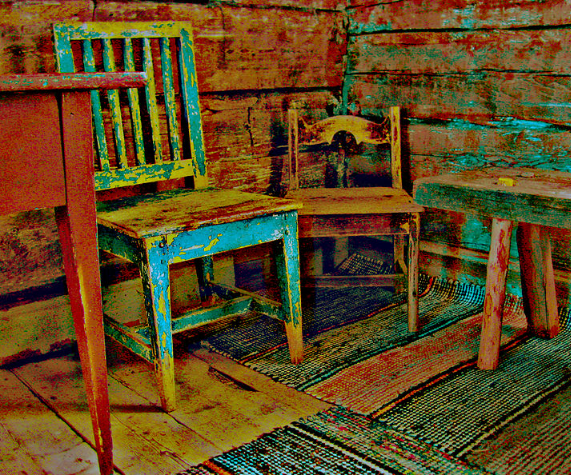
\includegraphics[width=.7\textwidth]{./imgs/art5.png}
\end{center}

\noindent\emph{Sente-se}, de Carulmare, é uma fotografia que foi tirada em 2009
e editada por meio do \textbf{paint.net}. Paint.net é um aplicativo gratuito para a manipulação e a edição de imagens e fotografias.

Com base na imagem e no texto, o desafio é você fazer arte por meio de uma
fotografia digital. Para isso, você vai precisar de:

\begin{itemize}
\item
  um aparelho de celular e algum aplicativo para tratamento da
  fotografia;
\item
  uma impressora para fazer uma cópia em papel da fotografia;
\item
  determinar, junto com a turma, o tema da exposição;
\item
  definir, junto com a turma, como montar a exposição das fotografias
  digitais para a comunidade escolar.
\end{itemize}

\begin{center}
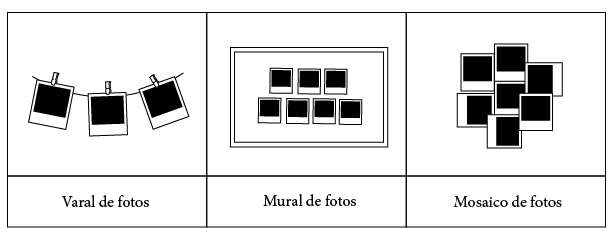
\includegraphics[width=.95\textwidth]{../ilustracoes/ART5/SAEB_5ANO_ART_FIGURA5.png}
\end{center}

% \coment{A escolha de um tema para a exposição amplia os olhares na fruição dessa
% manifestação e a capacidade de simbolizar. São exemplos de temas que
% podem fazer parte de uma exposição com foco no olhar do fotógrafo: “Da
% janela da minha casa”; “Eu de cima ou eu de baixo”; “Minha comunidade”.
% Existem muitos aplicativos para tratamento de fotografias disponíveis na
% internet e, possivelmente, os alunos já tiveram acesso a algum
% deles. Verifique com eles se já conhecem algum aplicativo, peça a ele que digam qual
% indicariam e que justifiquem a indicação. Sugerimos que escolham juntos
% apenas um aplicativo, para que as possibilidades de intervenção
% artística sobre a foto sejam as mesmas para todos. Alguns aplicativos disponíveis são: Snapseed, Lightroom e VSCO.}

\pagebreak
\num{8}

\begin{figure}[htpb!]
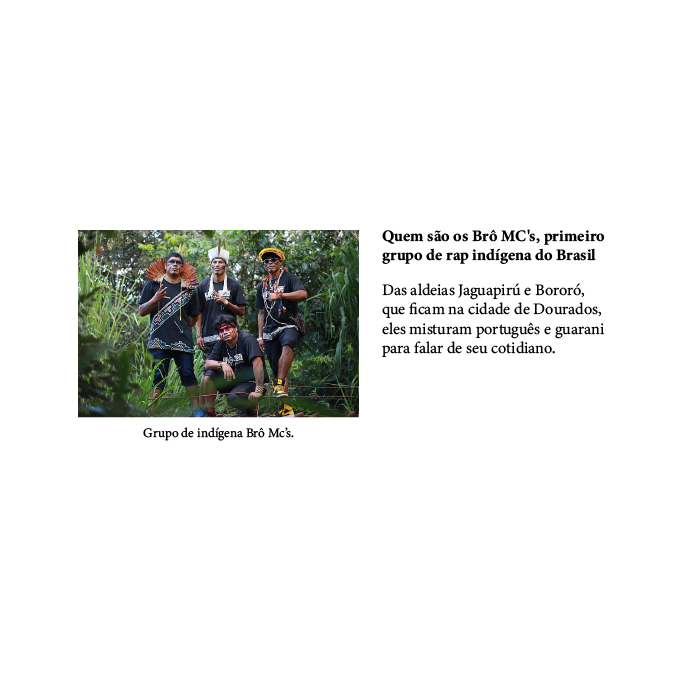
\includegraphics[width=\textwidth]{../ilustracoes/ART5/SAEB_5ANO_ART_FIGURA6.png}
\end{figure}

Quatro indígenas Guarani Kaiowá fundaram o primeiro grupo
de rap indígena do Brasil: o Brô MC's. De início, eles enfrentaram
a estranheza do público com a ideia de o ritmo ser apropriado pela
etnia, além de enfrentarem, dentro do próprio povoado, os caciques
questionando a empreitada. Agora, ouça – pelo menos duas vezes –
a música \textit{Terra vermelha}, do Brô MC's, disponível em: \emph{https://www.youtube.com/watch?v=ZwuM0z1IJWo} (acesso em: 19 mar. 2023).
Agora, interprete a letra da canção e, no espaço a seguir, escreva o
que para você é a temática da música.


\reduline{A música fala de questões indígenas importantes: a demarcação e a perda de terras.\hfill}
\linhas{10}

\pagebreak
\num{9} Leia a sinopse do espetáculo teatral infantil \emph{Pinocchio, o musical}.

\begin{myquote}
Com roteiro adaptado de um dos maiores clássicos de todos os tempos, o
espetáculo teatral infantil \textit{Pinocchio, o musical} traz uma releitura
contemporânea, que despertará interesse das crianças pela abordagem de
temas relacionados a educação, respeito, obediência aos pais, tudo de
uma forma lúdica, bem humorada e emocionante.

“Como inovação no mercado de peças infantis, trouxemos toda a
ambientação em projeções com realidade virtual, desenvolvidas por um dos
profissionais mais renomados do mercado”, salienta o diretor Luiz
Marcelo Legey.

“Após uma extensa pesquisa, estamos produzindo um musical com roteiro
adaptado de um dos mais tradicionais contos infantis, trazendo cenas e
diálogos contemporâneos, além de reunir uma equipe comprometida com o
objetivo da peça, trazendo muita diversão e uma experiência audiovisual
incrível”, reforçam as diretoras e roteiristas Ana Ferguson e Solange
Bighetti.

{[}\ldots{}{]}

\fonte{Pinnochio, o musical. Rio no teatro. Disponível em: \emph{https://www.rionoteatro.com.br/pinocchioomusical}.
Acesso em: 19 mar. 2023.}
\end{myquote}

Associe o termo ou a expressão do texto com seu significado.

\begin{center}
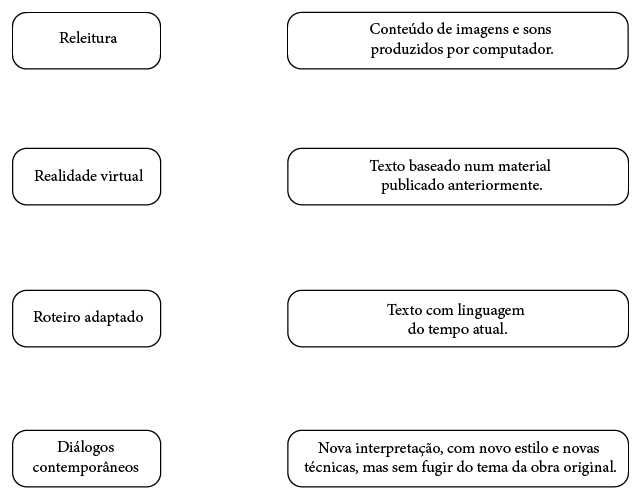
\includegraphics[width=.8\textwidth]{../ilustracoes/ART5/SAEB_5ANO_ART_FIGURA7.png}
\end{center}

% \coment{Releitura/nova interpretação, com novo estilo e novas
% técnicas, mas sem fugir do tema da obra original. Realidade virtual/
% Conteúdo de imagens e sons produzidos por computador. Roteiro adaptado/
% Texto baseado num material publicado anteriormente. Diálogos
% contemporâneos/ Texto com linguagem do tempo atual.}

\num{10} Utilizando quadrados, círculos e triângulos, crie, em uma folha à parte,
uma obra que represente um objeto, uma pessoa ou um animal. Vale utilizar uma fotografia como referência.

% \coment{Resposta pessoal.}

\section*{Treino}

\num{1} Observe a imagem e leia a legenda.

\begin{figure}[htpb!]
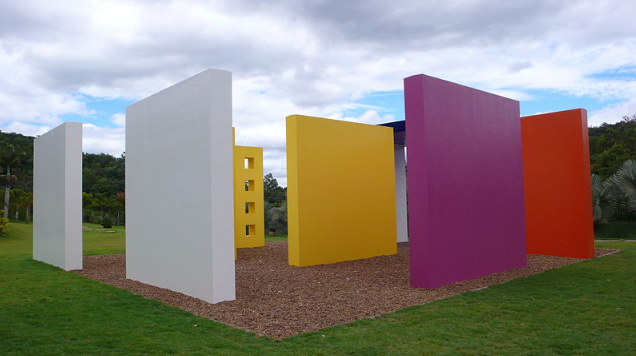
\includegraphics[width=\textwidth]{./imgs/art9.png}
\caption{\emph{Invenção da Cor}, \emph{Penetrável Magic Square \#5, De Luxe} (1977), de Hélio Oiticica. Pintura sobre paredes de alvenaria, cobertura de metal e vidro, alambrado, seixo rolado, 15m x 15m x 4,5m.Instituto Cultural Inhotim, Brumadinho, Minas Gerais.}
\end{figure}

Assinale a alternativa que corresponde a uma característica da obra.

\begin{escolha}
\item
  Obra colecionável.
\item
  Espaço bidimensional.
\item
  Espaço tridimensional.
\item
  Trabalho em pequeno formato.
\end{escolha}


\pagebreak
\num{2} Assinale a alternativa que descreve funções do orientador de público em museus.

\begin{escolha}
\item
  Responsável por dar informações para o público sobre as obras
  expostas, em visitas agendadas ou espontâneas.
\item
  Responsável por conservar e restaurar objetos do museu.
\item
  Responsável por pesquisar, classificar e analisar documentos e objetos
  do passado.
\item
  Responsável por supervisionar as áreas expositivas e informar as
  regras de comportamento no museu.
\end{escolha}



\num{3}  Leia o texto.

\begin{myquote}
Gênero musical e dança realizada com as canções desse ritmo, pode ser considerado um dos
grandes símbolos da cultura brasileira. E é um patrimônio imaterial do Brasil, além de
ser muito popular no exterior. Surgido no Rio de Janeiro, no começo do século XX, é
resultado da influência da cultura africana no Brasil. O surgimento desse ritmo se deu
nos encontros de afro-brasileiros reunidos para celebrar sua cultura.
\end{myquote}

Assinale a alternativa que corresponde ao gênero musical descrito no texto.

\begin{escolha}
\item
  Hip-hop.
\item
  Rock.
\item
  Samba.
\item
  Sertanejo.
\end{escolha}


\chapter[O corpo na arte, a arte no corpo, a arte do corpo]{\Large O corpo na arte, a arte no corpo,\\ a arte do corpo}
\markboth{Módulo 2}{}

\vspace*{-1\baselineskip}

\section*{Habilidades do SAEB}

\begin{itemize}
\item Identificar as características de instrumentos musicais variados, bem
como o potencial musical do corpo humano.

\item Reconhecer diferentes formas de notação musical.

\item Reconhecer a influência de distintas matrizes estéticas e culturais
nas manifestações das artes visuais, dança, música e teatro na cultura
brasileira.

\item Analisar expressões do teatro e da dança na vida cotidiana.

\item Analisar relações entre as partes corporais e seu todo na estética da dança.
\end{itemize}

\subsection{Habilidade da BNCC}

\begin{itemize}
\item EF15AR03.
\end{itemize}

\conteudo{
\begin{wrapfigure}{l}{.5\textwidth}
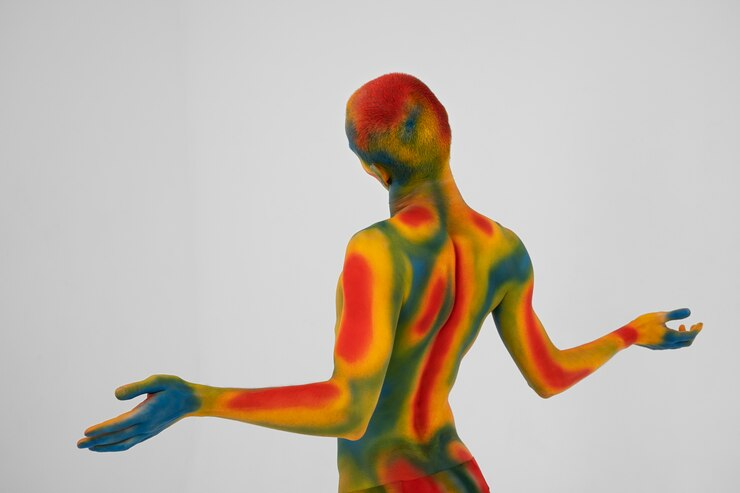
\includegraphics[width=.5\textwidth]{./imgs/art40.jpg}
\caption{Artista com o corpo pintado.}
\end{wrapfigure}

Você já parou para pensar na importância do corpo para a arte?

O \textbf{corpo na arte} pode ser, por exemplo, qualquer manifestação
das artes visuais em que o corpo humano esteja representado. Pode ser
uma pintura, uma escultura, um desenho, uma fotografia, um artesanato,
uma xilogravura.

A \textbf{arte no corpo} pode ser uma tatuagem, uma pintura corporal
indígena, uma máscara, uma fantasia.

Já a \textbf{arte do corpo} pode ser encontrada nas pessoas que dançam,
fazem mímica, realizam percussão com o corpo ou representam personagens.

Para compreender essas relações do corpo com a arte, precisamos entender
que toda manifestação artística faz parte de um momento histórico e
cultural de uma comunidade, região ou país. Desse modo, é preciso pensar:
quais eram ou são as crenças, os saberes, as técnicas disponíveis?

Para você ampliar seus conhecimentos sobre a arte, é necessário ter experiências artísticas
sensíveis, investigando a diversidade presente nas manifestações e refletindo sobre isso
seja como apreciador/interlocutor, como criador.}


\section*{Atividades}

Para responder às atividades de 1 a 3, leia o texto.

\begin{myquote}
O corpo humano é uma fonte muito rica de sons e pode ser considerado
nosso primeiro instrumento musical. Sentimos a presença do ritmo na
batida de nosso coração, em nossa respiração ou ao caminharmos.
Reconhecemos inúmeros timbres e melodias na exploração de nossa voz e
também na escuta da voz do outro. {[}\ldots{}{]}

Ao redor do mundo, observa-se uma rica diversidade de formas de canto,
de palmas, de estalos de dedo, de estalos de língua, de sapateados, de
assobios, além dos sons vocais, fonéticos (sons da fala) e onomatopaicos
(reproduz sons de animais, da natureza, entre outros), que conferem à
língua falada de cada região o seu sotaque particular. Essa música
corporal está presente no dia a dia das comunidades, assim como nas suas
danças e festividades. No Brasil existem inúmeros estilos musicais que
se utilizam de sapateados e de palmas em suas manifestações, como: o
coco, o xaxado, o samba de roda, a catira, a chula e o fandango, cujas
coreografias por si só têm um resultado rítmico. {[}\ldots{}{]}

\fonte{Disponível em:
\emph{http://www.abemeducacaomusical.com.br/revista\_musica/ed5/artigo3.pdf.}
Acesso 20 mar. 2023. (Adaptado para fins didáticos.)}
\end{myquote}

\num{1}  O corpo humano pode ser considerado uma fonte de sons, podendo, inclusive, ser comparado a nosso primeiro instrumento musical. Pesquise exemplos de manifestações artísticas brasileiras
  em que as próprias coreografias se utilizam da música corporal? Registre a seguir.

\reduline{São exemplos: coco, xaxado, samba de roda, catira, chula e fandango. Após a realização da atividade, divida a turma em seis grupos, e cada grupo
será responsável por pesquisar uma manifestação artística diferente entre esses exemplos citados.
Marque com eles um dia para que os grupos apresentem suas descobertas.
Oriente-os sobre as informações que não podem faltar na pesquisa: as
matrizes históricas e culturais (como se faz presente a matriz africana,
indígena ou europeia), os instrumentos musicais que fazem parte dessa
manifestação e como o corpo é utilizado para produzir sons.
Vídeos são importantes nesse tipo de pesquisa. Sugestões: \emph{Coco de Roda Sucena Maringá}, disponível em: \emph{https://bit.ly/2MOMEDZ}; \emph{Tropeiros da Borborema}, disponível
em: \emph{https://bit.ly/3VDcleP}; \emph{Vídeo Grupo Sucena} \emph{– Samba De Roda:} \emph{Ritmos e Manifestações} \emph{Afro-Brasileiras}, disponível em: \emph{https://bit.ly/3NLWBnY};
\emph{Araguaia presente de} \emph{Deus}, disponível
em: \emph{https://bit.ly/3HLJpfe}; \emph{Alma Gaúcha} , disponível em: \emph{https://bit.ly/42hxQ7J}; \emph{Extras Documentário} \emph{Fandango}, disponível em: \emph{https://bit.ly/3B4jJX9}. Acessos em: 20 mar. 2023.
Quando a pesquisa estiver concluída, cada grupo poderá organizar em uma
folha avulsa as informações e, depois, tirar cópias dessas informações
para os colegas dos outros grupos. Assim, ao final, a turma terá dados
de todas as manifestações pesquisadas.\hfill}

\num{2}  Você vai seguir as instruções a seguir e produzir sons com o corpo.


\conteudo{
\begin{itemize}
\item\textbf{Bata palma com as costas da mão}: feche uma das mãos e bata as costas
  da mão fechada na palma da outra mão.\bigskip

   \item\textbf{Faça estalos com os dedos}: deslize o polegar pelo dedo médio,
  deixando que este dedo bata contra a parte inferior do outro dedo.\bigskip

   \item\textbf{Bata a palma estrela}: abra bem as duas mãos e bata uma contra
  a outra.\bigskip

   \item\textbf{Bata no peito}: abra as mãos e bata as duas, alternadamente,
  contra cada um dos lados do peito.\bigskip

   \item\textbf{Bata na barriga}: abra as mãos e bata cada uma delas, alternadamente,
  contra um dos lados da barriga.\bigskip

   \item\textbf{Bata nas coxas}: com as mãos abertas, bata em cada uma das coxas.\bigskip

 \item\textbf{Faça estalo com os lábios}: feche bem os lábios e, em um movimento
  rápido, abra-os bem, fazendo um estalo.\bigskip

   \item\textbf{Faça barulho com beijo}: estale os lábios dando um beijo no ar.\bigskip

 \item\textbf{Faça estalo com a língua}: com a boca aberta, deslize a língua
  pelo palato, fazendo um estalo.
\end{itemize}
  }

% \coment{Faça com que os alunos, em roda, treinem um som de cada
% vez, para que possam perceber se o som é agudo ou grave, forte ou fraco,
% ou se pode ser executado de forma rápida ou lenta, por exemplo.
% A seguir, peça que os alunos executem a sequência de sons e movimentos
% do corpo duas vezes, ou seja, duas palmas costas de mão, dois estalos de
% dedos, duas palmas estrela, e assim por diante. A seguir, peça que
% realizem sequência de três e depois de quatro. Essas sequências podem
% começar com movimentos lentos e depois cada vez mais rápidos.}

\num{3}  A partitura a seguir é para ser interpretada por você junto com seus
  colegas de turma. Para isso, será necessário memorizar o significado
  de cada símbolo.

\begin{figure}[htpb!]
\centering
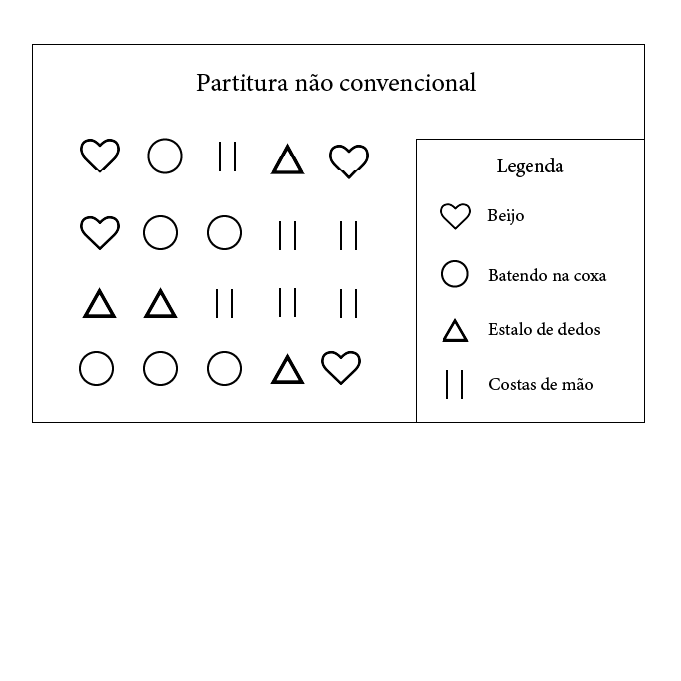
\includegraphics[width=\textwidth]{../ilustracoes/ART5/SAEB_5ANO_ART_FIGURA11.png}
\end{figure}

% \coment{Relembre seus alunos que, na partitura, assim como nos textos escritos,
% lemos em linhas horizontais, da esquerda para a direita e de cima para
% baixo.}

\pagebreak
\num{4}  Complete o esquema a seguir.

\begin{figure}[htpb!]
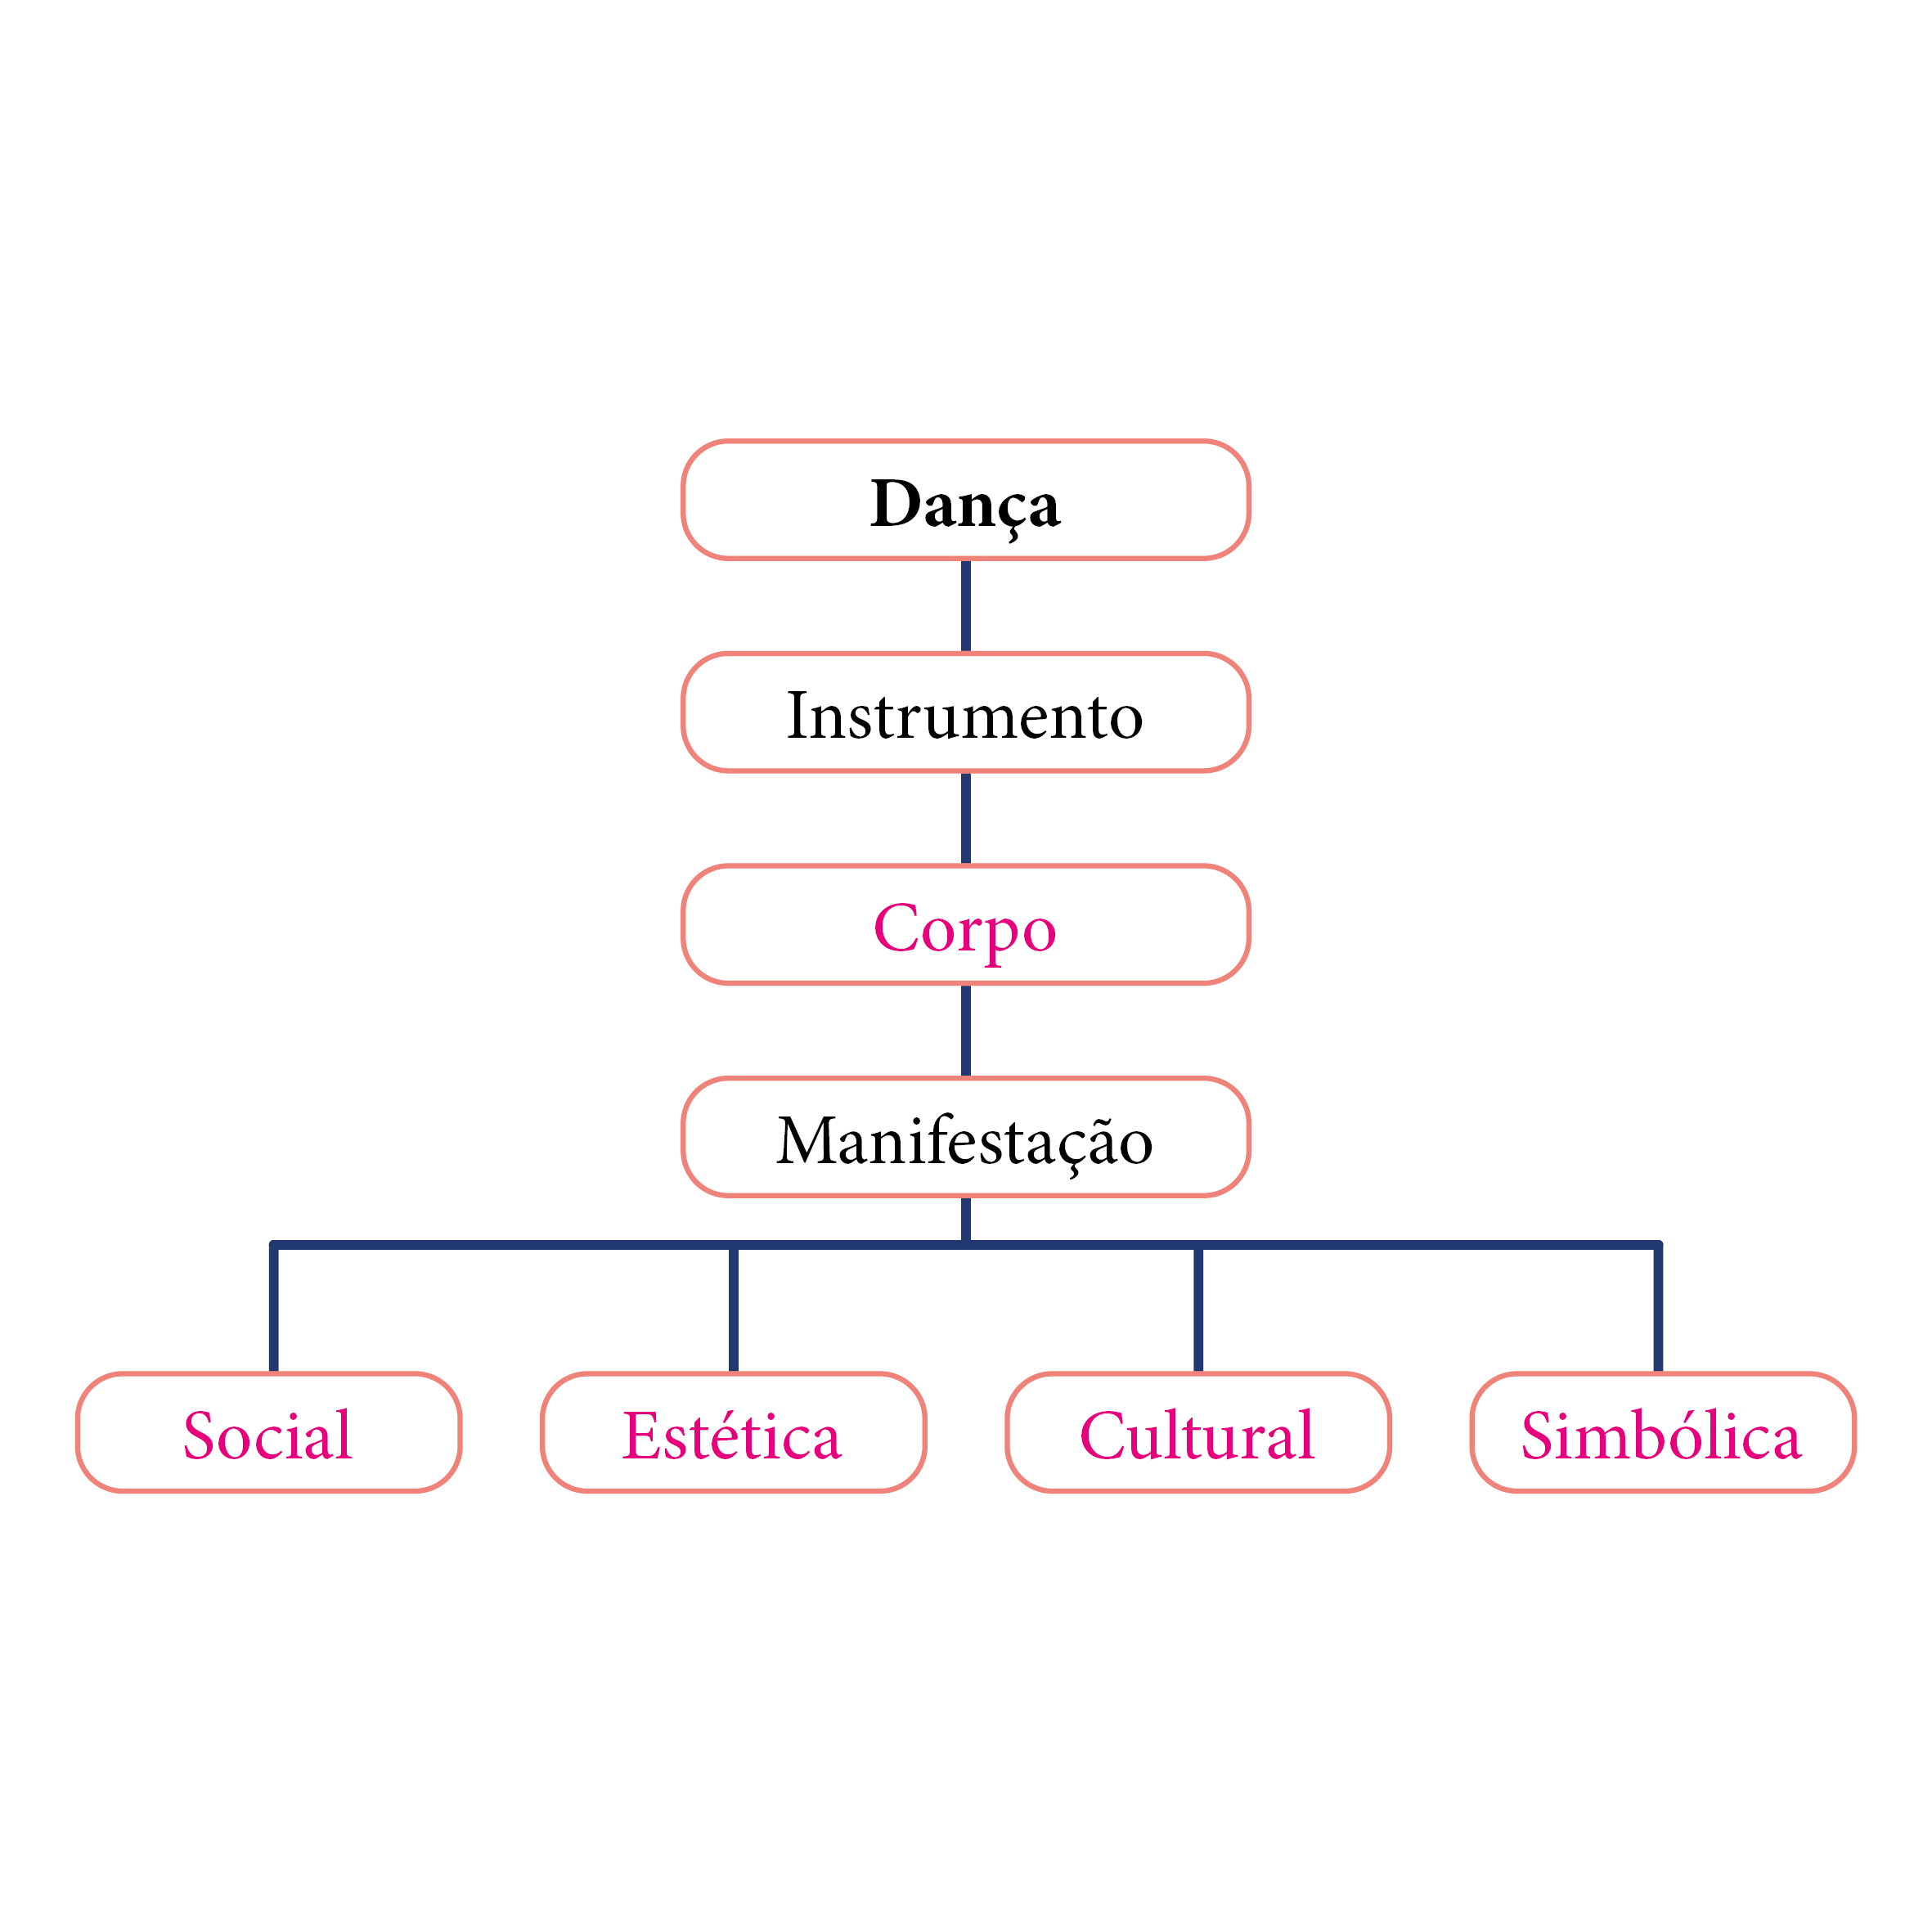
\includegraphics[width=\textwidth]{../ilustracoes/ART5/SAEB_5ANO_ART_FIGURA12.png}
\end{figure}


\num{5}  Associe a descrição do passo de balé à sua imagem.

\begin{mdframed}[linewidth=2pt,linecolor=salmao,backgroundcolor=salmao!20]
\textbf{1. Cambré} – Arqueado.\\
Dobrar o corpo a partir da cintura, para a frente, para trás ou para os
lados, a cabeça acompanha o movimento.

\bigskip
\noindent\textbf{2. Jeté} – Jogado, atirado.\\
Um pulo de uma perna para qualquer direção.

\bigskip
\noindent\textbf{3. Arabesque} – Arabesco.\\
É uma das poses básicas do ballet, onde o bailarino fica apoiado numa só
perna que pode estar na vertical ou em demi plié, com a outra perna
estendida para trás e em ângulo reto com ela, sendo que os braços estão
estendidos em várias posições harmoniosas criando a linha mais longa
possível da ponta dos dedos da mão à dos pés. Os ombros devem ser
mantidos retos em frente à linha de direção.

\bigskip
\noindent\textbf{4. Derriére} – Atrás.\\
Movimento, passo ou a colocação de um membro atrás do corpo.
\end{mdframed}

\pagebreak
\begin{figure}[htpb!]
\acima{(\rosa{2}) \hfill(\rosa{3})}
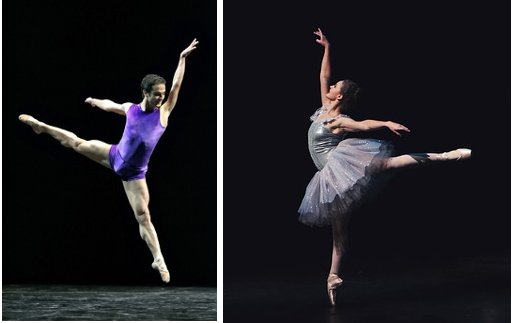
\includegraphics[width=\textwidth]{./imgs/art15ab.png}
\end{figure}

\begin{figure}[htpb!]
\acima{(\rosa{4}) \hfill(\rosa{1})}
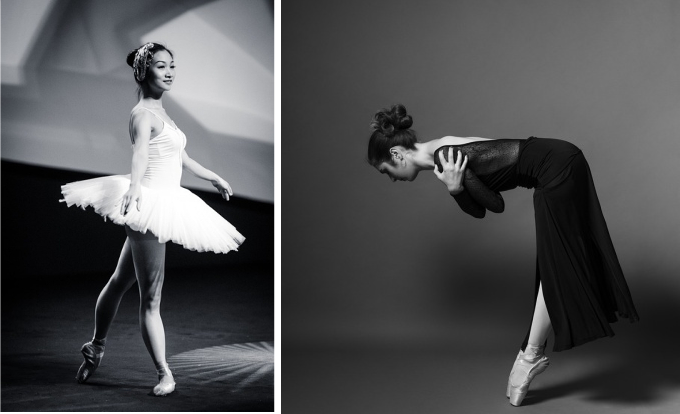
\includegraphics[width=\textwidth]{./imgs/art15cd.png}
\end{figure}

%Fonte: \emph{https://escolaartedanca.com.br/dicionario-de-ballet}. Acesso
%em: 20 mar. 2023.

% \coment{Informe aos seus alunos que os nomes das técnicas do balé clássico e 
% os nomes dos passos, das ações e das mímicas são do francês. Os franceses
% foram os primeiros a codificar as técnicas, e essa tradição se mantém até
% os dias atuais.}

\pagebreak
Para responder às atividades 6 e 7, leia o texto.

\begin{myquote}
Fundada em 1979, a trupe teatral \emph{Esquadrão da vida}, de Brasília,
foi pioneira em abordar o resgate e a valorização da cultura popular, a
denúncia da exclusão de parte da população dos espaços culturais tradicionais,
a subversão bem-humorada do espaço público e a conscientização ecológica.
A trupe faz um teatro que é livre de academicismo e emprega elementos
expressivos das festas populares, além de acobacia, música e dança.
acrobacia, música e dança. Em Brasília, uma cidade administrativa,
a importância do teatro de rua é gigantesca.

\fonte{Fonte de pesquisa: Esquadrão da vida. Disponível em:
\emph{https://brasilia.memoriaeinvencao.com/esquadrao-da-vida}. Acesso
em: 21 mar. 2023.}
\end{myquote}

\num{6}  Responda aos itens a seguir.

\begin{escolha}
\item Quais são os temas abordados pela trupe teatral Esquadrão da vida?\\
\reduline{Resgate e valorização da cultura popular; denúncia da exclusão de
parte da população dos espaços culturais tradicionais; subversão bem-humorada
do espaço público; conscientização ecológica.\hfill}

\item Qual é o formato da arte produzida pela trupe teatral Esquadrão da vida?\\
\reduline{Teatro de rua.\hfill}

\item Que elementos a trupe Esquadrão da vida incorpora ao teatro?\\
\reduline{Festas populares, acrobacia, música e dança.\hfill}
\end{escolha}

\num{7} Qual é o perfil do público que participa de uma apresentação de teatro em espaços públicos e abertos?

\reduline{Resposta pessoal. É esperado que os alunos compreendam que todas as
pessoas que passam pela rua, que não foram convidadas, não compraram
ingressos, mas se depararam com a apresentação no seu cotidiano, participal do teatro de rua.
São espectadores/participantes ativos, de todas as idades, gêneros, etnias, classes sociais.\hfill}

\pagebreak

Para resolver as atividades 8 e 9, leia o texto.\bigskip

\begin{myquote}
\textbf{Cultura: Saiba mais sobre o maracá}

O maracá é um dos instrumentos musicais indígenas mais conhecidos, sendo
seu nome muitas vezes utilizado como uma designação genérica para
chocalhos. Consiste numa cabaça seca e oca com pequenas pedras, caroços
ou sementes em seu interior, colocada na extremidade de um bastão,
normalmente feito de madeira.

\begin{wrapfigure}{l}{.5\textwidth}
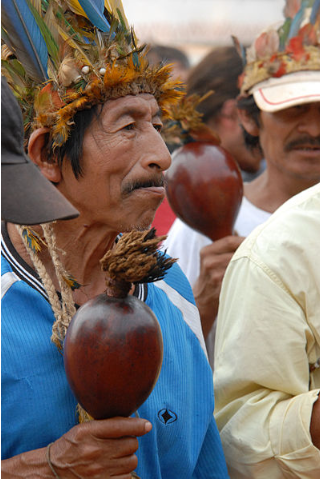
\includegraphics[width=.5\textwidth]{./imgs/art18.png}
\caption{Karai Guarani com Maracá}
\end{wrapfigure}
%\emph{https://commons.wikimedia.org/wiki/File:Xam\%C3\%A3_guarani.jpg}

Em determinados casos, o instrumento é atravessado pela haste e
apresenta dois cabos. Alguns maracás são ornamentados com penas no
suporte e outros têm a cabaça ornada com desenhos. Entre as mais
diversas populações indígenas, o maracá é utilizado geralmente para
marcar o ritmo do canto e da dança durante cerimônias, festividades,
ritos e outras manifestações culturais e sociais.


\textls[-10]{Há etnias que acreditam que o maracá possui grande poder espiritual. Considerado um objeto nobre, é também utilizado pelos pajés em solenidades e rituais religiosos. Algumas comunidades, por exemplo, acreditam que os espíritos falam por meio dos maracás. O poder sobrenatural do artefato é devido não apenas ao som misterioso produzido pelos grãos e pedras nele contidos, mas também pelas pinturas e gravuras que enfeitam o instrumento sonoro.}\looseness=-1

\fonte{Fundação Nacional dos Povos Indígenas. Cultura: Saiba mais sobre o maracá, instrumento musical indígena.
Disponível em: \emph{https://www.gov.br/funai/pt-br/assuntos/noticias/2022-02/cultura-saiba-mais-sobre-o-maraca-instrumento-musical-indigena}.
Acesso em: 21 mar. 2023.}
\end{myquote}

\pagebreak
\num{8}  Complete a tabela com informações retiradas do texto.\bigskip

\noindent\resizebox{!}{.1\textwidth}{
\begin{tabular}{|ll|}
\hline
\multicolumn{2}{|c|}{\textbf{Maracá – instrumento musical de origem indígena}} \\ \hline
\multicolumn{1}{|c|}{\textbf{Material utilizado na confecção}} & \multicolumn{1}{c|}{\textbf{Para que é utilizado}} \\ \hline
\multicolumn{1}{|l|}{\rosa{cabaça}} & \multirow{4}{*}{\begin{tabular}[c]{@{}l@{}}\rosa{Para marcar o ritmo do canto e da dança durante cerimônias,}\\ \rosa{festividades, ritos e outras manifestações culturais e sociais.}\end{tabular}} \\
\multicolumn{1}{|l|}{\rosa{pedras, caroços ou sementes}} &  \\
\multicolumn{1}{|l|}{\rosa{madeira}} &  \\
\multicolumn{1}{|l|}{\rosa{penas}} &  \\ \hline
\end{tabular}
}

\num{9}  Assinale a alternativa que corresponde à forma como o som do maracá é produzido.

\begin{boxlist}
\boxitem{\white{X}} Instrumento que soa pela vibração do ar no seu interior.

\boxitem{\white{X}} Instrumento que soa pela vibração de uma membrana esticada em algum suporte.

\boxitem{X} Instrumento que soa pela própria vibração do instrumento.

\boxitem{\white{X}} Instrumento que soa pela vibração de cordas tensionadas.
\end{boxlist}


\num{10} Leia a descrição de um instrumento.

\begin{myquote}
Instrumento musical importantíssimo no Brasil, utilizado em músicas
de pagode e samba, por exemplo. Foi trazido para o Brasil pelos portugueses
e passou a ser muito usado, na capoeira, pelos escravizados.
\end{myquote}

Assinale a imagem que representa o instrumento musical correspondente à descrição.

\begin{figure}[htpb!]
\acima{( ) \hfill(\rosa{X})}
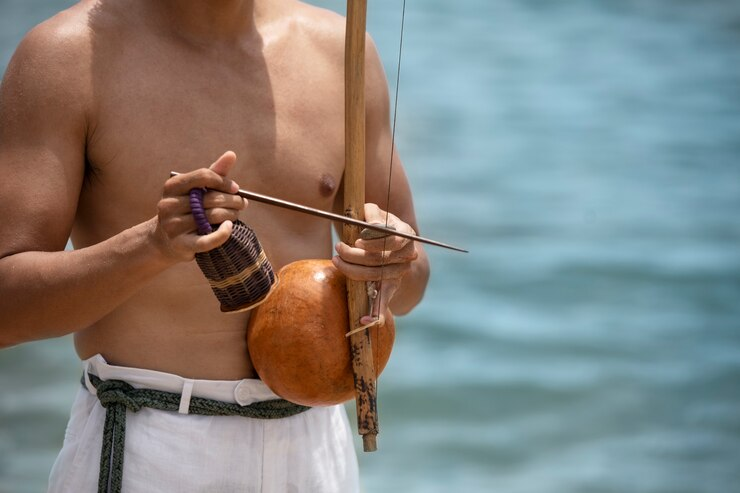
\includegraphics[width=.5\textwidth]{./imgs/art19a.jpg}
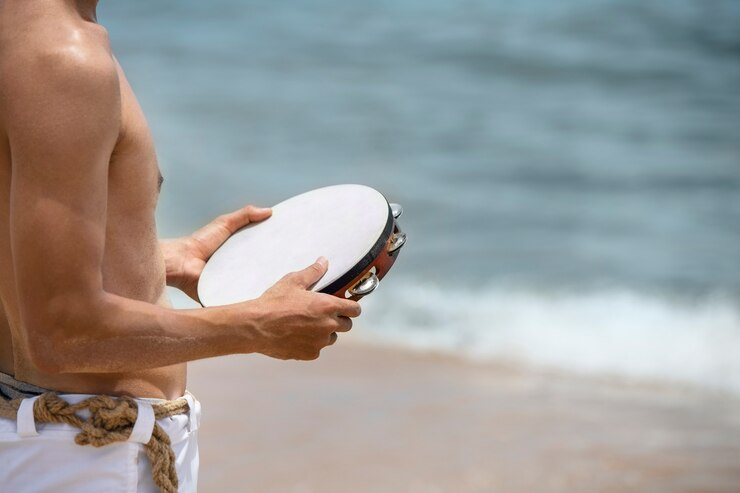
\includegraphics[width=.5\textwidth]{./imgs/art19b.jpg}
\caption{Berimbau e pandeiro}
\end{figure}

\begin{figure}[htpb!]
\acima{( ) \hfill( )}
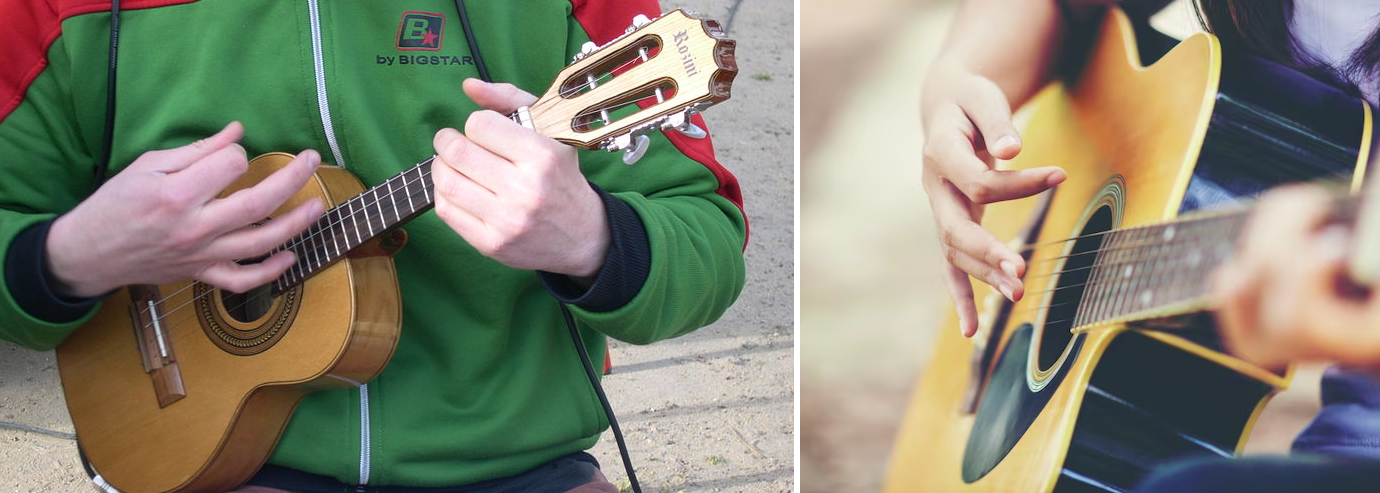
\includegraphics[width=\textwidth]{./imgs/art19cd.png}
\caption{Cavaquinho e violão}
\end{figure}

\section*{Treino}

\num{1} Leia o texto.

\begin{myquote}
\textbf{Balé clássico}

Foi Charles-Louis-Pierre de Beauchamps, o primeiro grande ``maître de ballet'', no século XVII, que criou as cinco posições básicas no balé, criadas para manter o equilíbrio do corpo em movimento ou parado e organizar a estética da dança.

\fonte{Fonte de pesquisa: Secretaria da Educação. Balé clássico. Disponível em: \emph{http://www.arte.seed.pr.gov.br/modules/conteudo/conteudo.php?conteudo=135}. Acesso em: 04 abr. 2023.}
\end{myquote}

Assinale a alternativa que apresenta características técnicas do balé
clássico no Brasil e no mundo.

\begin{escolha}
\item
  Na prática do balé, o excesso de exercícios e repetições pode causar
  lesões em ossos e músculos.
\item
  No balé, são utilizados dois tipos de sapatilha: a “de meia ponta” e
  a “de ponta”.
\item
  O balé clássico surgiu no século XV e fazia parte do entretenimento
  dos nobres italianos.
\item
  O bale clássico é uma modalidade de dança que, geralmente, segue o
  mesmo padrão de posições no Brasil e em qualquer parte do mundo.
\end{escolha}



\pagebreak
\num{2} Observe a imagem.

\begin{figure}[htpb!]
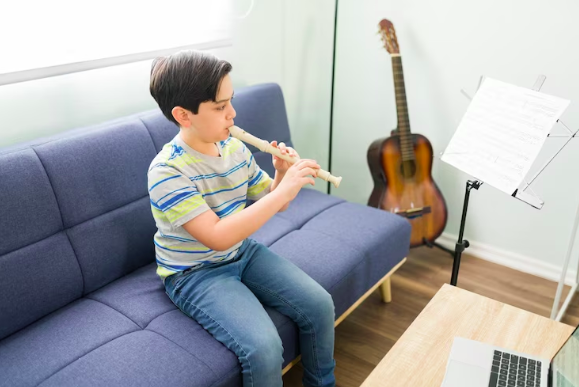
\includegraphics[width=\textwidth]{./imgs/art41.png}
\end{figure}

Na imagem, um garoto toca um instrumento conhecido como flauta. Em um instrumento como esse, o som é produzido pela vibração

\begin{escolha}
\item
  do instrumento em si.
\item
  de cordas tensionadas.
\item
  de uma membrana esticada em algum suporte.
\item
  do ar no interior do instrumento.
\end{escolha}



\pagebreak
\num{3}  Leia o texto.

\begin{myquote}
\textbf{Samba de Roda do Recôncavo baiano passa a ser Patrimônio Imaterial do Estado}

{[}\ldots{}{]}

O Samba de Roda do Recôncavo Baiano é um misto de expressão musical,
coreografia característica, poética abrangente, presente em momentos
festivos. É uma das principais manifestações culturais engendradas em
solo brasileiro. {[}\ldots{}{]}

Seus primeiros registros, com esse nome e com muitas características que
ainda hoje o identificam, datam dos anos 1860. Atualmente, reúne as
tradições culturais transmitidas por africanos escravizados e seus
descendentes, que incluem o culto aos orixás e caboclos, o jogo da
capoeira e a chamada comida de azeite. A herança negro-africana no samba
de roda se mesclou de maneira singular a traços culturais trazidos pelos
portugueses (principalmente viola e pandeiro) e à própria língua
portuguesa nos elementos de suas formas poéticas.

{[}\ldots{}{]}

\fonte{SECULTBA. Samba de Roda do Recôncavo baiano passa a ser Patrimônio Imaterial do Estado.
Disponível em: \emph{http://www.cultura.ba.gov.br/2020/03/17464/Samba-de-Roda-do-Reconcavo-baiano-passa-a-ser-Patrimonio-Imaterial-do-Estado.html}.
Acesso em: 21 mar. 2023.}
\end{myquote}

A principal matriz estética e cultural do Samba de Roda do Recôncavo Baiano é a

\begin{escolha}
\item
  africana.
\item
  asiática.
\item
  europeia.
\item
  indígena.
\end{escolha}


\chapter{Patrimônio cultural}
\markboth{Módulo 3}{}

\vspace*{-1.5cm}
\enlargethispage{2\baselineskip}

\section*{Habilidade do SAEB} \enlargethispage{2\baselineskip}

\begin{itemize}
\item Avaliar nas linguagens artísticas a diversidade do patrimônio cultural
da humanidade (material e imaterial), em especial o brasileiro, a partir
de suas diferentes matrizes.
\end{itemize}

\subsection{Habilidade da BNCC}

\begin{itemize}
\item EF15AR25.
\end{itemize}

\conteudo{Observe cada uma das imagens a seguir.

\begin{center}
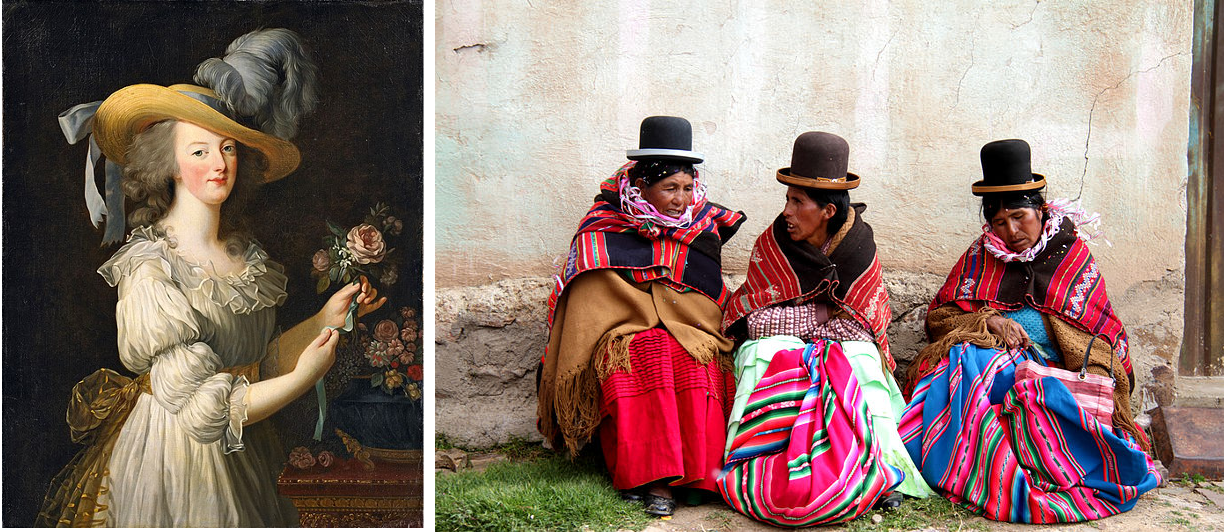
\includegraphics[width=.7\textwidth]{./imgs/art22ab.png}

Vestimenta do século XVIII -- Trajes típicos bolivianos
\end{center}

\begin{center}
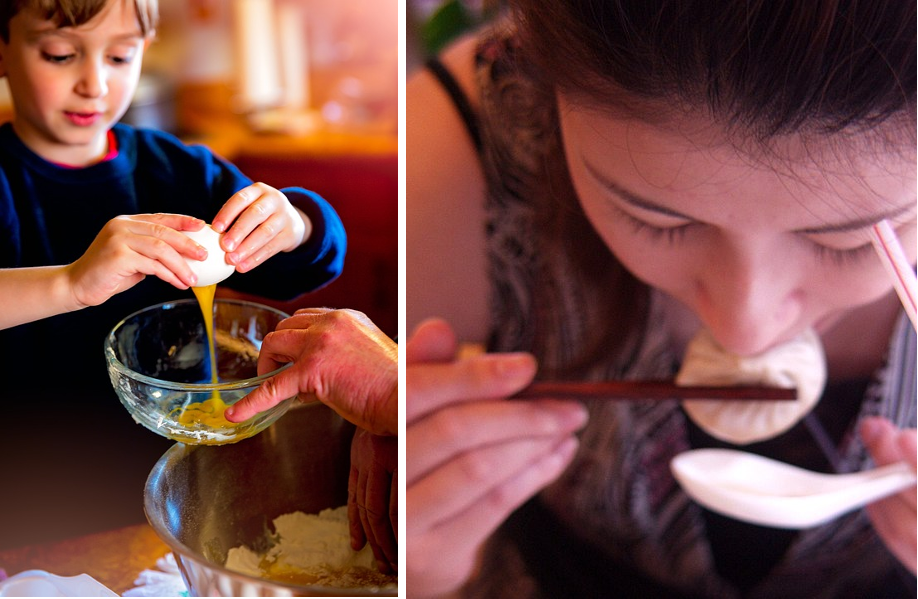
\includegraphics[width=.7\textwidth]{./imgs/art22cd.png}

Criança aprendendo a fazer pão de queijo com o pai -- Chinesa comendo com palitinhos
\end{center}
}

\conteudo{
\begin{minipage}{\textwidth}
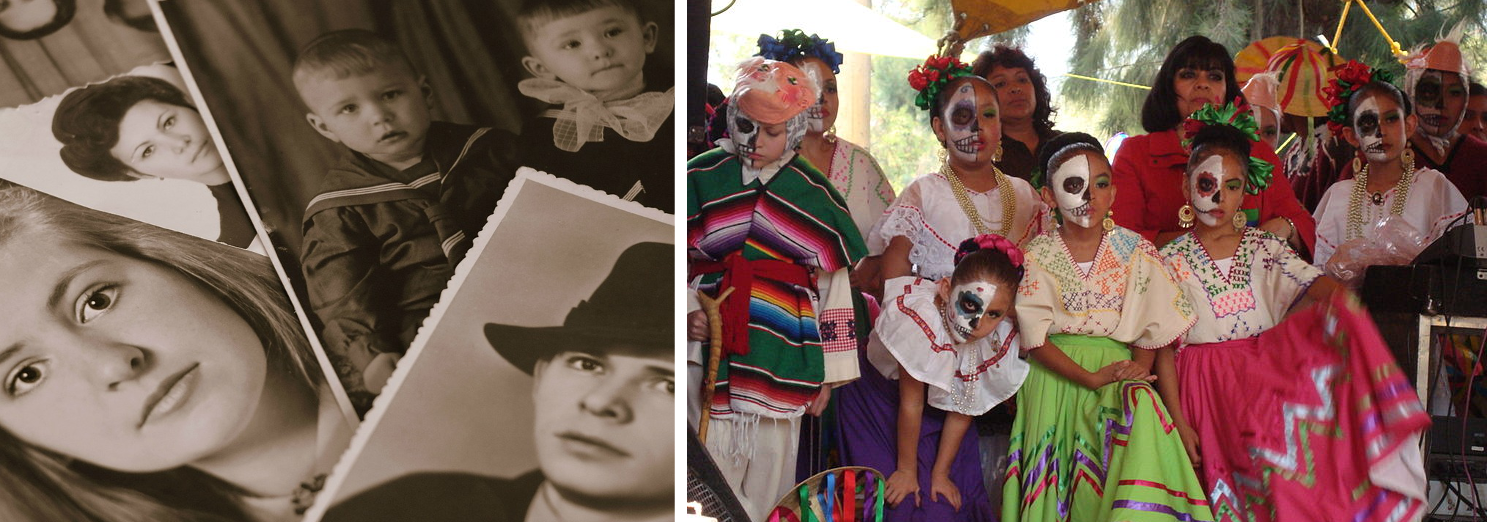
\includegraphics[width=\textwidth]{./imgs/art22ef.png}
\end{minipage}
\begin{minipage}{\textwidth}\vspace{.5cm}
Grupo mexicano de dança – Festa dos Mortos e fotos de família
\end{minipage}\bigskip

Você pôde observar e analisar trajes típicos de outro país, vestimenta do
século XVIII, palitinho típicos da China que funcionam como os nossos talheres,
image de uma festa mexicana. Além disso, você viu objetos, como fotografias que alguma pessoa
escolheu para guardar, e uma criança aprendendo o modo de
fazer pão de queijo.

Cada uma dessas imagens representa algo que pode fazer parte do patrimônio de uma pessoa, de
um grupo ou de um país e que revela detalhes de uma cultura, que compreende as visões de mundo, as crenças, os saberes e os
fazeres transmitidos de geração a geração. O patrimônio é tudo aquilo que escolhemos para guardar: histórias,
objetos, memórias.

Podemos unir essas duas ideias e dizer, de forma
simplificada, que o \textbf{patrimônio cultural} compreende os \textbf{bens materiais}
(que se podem tocar) e os \textbf{bens imateriais} (que não se podem tocar) que cada grupo,
região ou país escolheu para preservar, conservar e proteger.

\begin{itemize}
  \item São exemplos de bens materiais: fotografias, vestimentas, obras de arte,
cidades ou talheres típicos.

\item São exemplos de bens imateriais: culinária, danças,
festas ou lendas.
\end{itemize}
}

% \coment{Sugerimos que a primeira leitura do texto seja realizada por você e
% acompanhada pelos alunos, numa roda de conversa. Primeiro faça com que
% os alunos observem e analisem as imagens e as legendas, uma de cada vez,
% buscando encontrar diferenças e semelhanças com a cultura brasileira e
% contemporânea. Depois, leia um parágrafo de cada vez, discutindo com
% eles as ideias e as informações apresentadas. Ao final da conversa, abra
% espaço para que os alunos esclareçam suas dúvidas.}

\pagebreak
\section*{Atividades}

\num{1} Os marajoaras chegaram à atual Ilha de Marajó por volta do ano 400. A principal arte que produziam é a cerâmica, que podia ser de \textbf{uso doméstico}, sem superfície decorada, para guardar mantimentos, de \textbf{uso cerimonial}, com superfície bem decorada (com desenhos, cortes ou alto relevo), para ser aplicada em festas ou homenagens fúnebres, ou de \textbf{uso funeral}, com superfície decorada com desenhos labirínticos. Agora, observe a imagem abaixo.

\begin{figure}[htpb!]
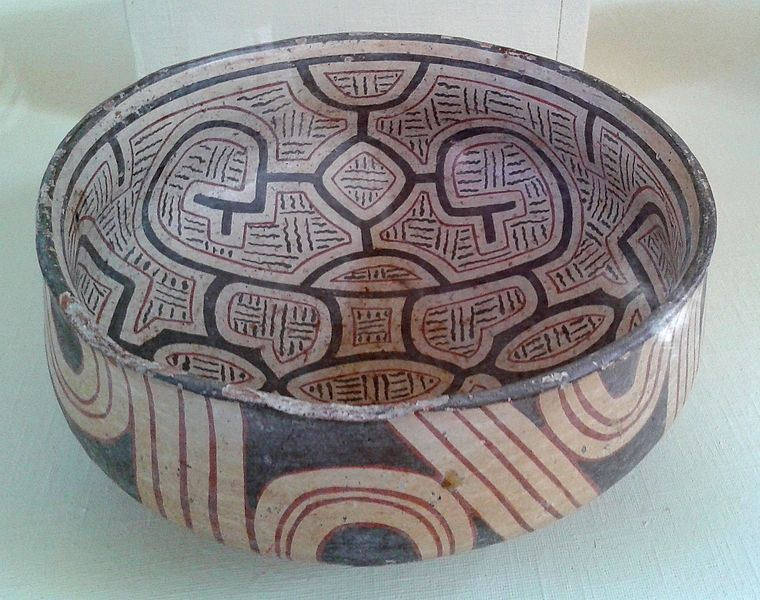
\includegraphics[width=\textwidth]{./imgs/art24.jpg}
\caption{Cerâmica marajoara. Acervo de arqueologia brasileira do Museu Nacional/UFRJ – Rio de Janeiro, Brasil.}
\end{figure}

\noindent{}A cerâmica representada nessa imagem devia ser de uso pessoal, cerimonial ou funeral? Justifique sua resposta.

\reduline{Essa cerâmica devia ser de uso cerimonial, pois é bem decorada e apresenta desenhos.\hfill}
\linhas{2}


\num{2}  Além da cerâmica, que outros patrimônios materiais a cultura marajoara nos deixou? Pesquise e responda.

\reduline{Bancos, colheres, apitos, adornos para orelha e lábios e estatuetas humanas.\hfill}
\linhas{3}


Para resolver as atividades 3 e 4, leia o texto.

\begin{myquote}
\textbf{Arte kusiwa}

Os wajapi pertencem ao grupo tupi-guarani e estão situados no norte da
Amazônia. Lá, existem cerca de 40 aldeias, totalizando 580 habitantes,
agrupadas em um território protegido do Estado do Amapá.

Há, entre os wajapi, uma tradição de utilizar tinturas vegetais vermelhas
(confeccionadas à base de uma planta amazônica conhecida como bija, além
de resinas perfumadas) para adornar, com motivos geométricos, os corpos e
outros objetos. Os motivos mais recorrentes são a onça-pintada, a cobra, a
borboleta e o peixe.

A arte kusiwa é a linguagem gráfica dos wajapi. Esse povo
desenvolveu uma linguagem que combina arte gráfica e verbal, refletindo uma
visão de mundo particular, por meio da qual são transmitidos os conhecimentos
essenciais da vida da comunidade.

Essa arte é considerada tão complexa que, para os wajapi, não é possível, antes
dos 40 anos de idade, conquistas as competências técnicas e artísticas necessárias
para dominar a arte do desenho e da preparação das tinturas. A arte kusiwa dá conta
da criação da humanidade e ilustra os mitos sobre o surgimento do ser humano.

\fonte{Fonte de pesquisa: iPatrimônio. Amapá – Arte Kusiwa. Disponível em:
\emph{https://www.ipatrimonio.org/amapa-arte-kusiwa/\#!/map=38329\&loc=1.1787550000000038,-52.767663,17}.
Acesso em: 22 mar. 2023.}
\end{myquote}


\num{3}  Qual é a visão dos wajapi sobre a complexidade da arte kusiwa?

\reduline{Os wajapi consideram não ser possível alcançar as competências técnicas
e artísticas necessárias para dominar a arte do desenho e da preparação
das tinturas antes dos 40 anos de idade.\hfill}
\linhas{2}

\pagebreak
\num{4}  Pesquise na internet uma imagem que represente uma manifestação da
arte kusiwa e cole-a no espaço a seguir.

\begin{mdframed}[linewidth=2pt,linecolor=salmao,roundcorner=20pt]
\coment{Resposta circunstancial.}
\vspace{19cm}
\end{mdframed}



Para resolver atividades 5 e 6, leia o texto.

\begin{myquote}
\textbf{Jogo de tabuleiro criado por indígenas empolga estudantes}\\
Em meio a tantas histórias e curiosidades em exposição durante a Semana
Nacional de Ciência e Tecnologia, em Brasília, eram as mesinhas com o
jogo da onça que mais capturavam estudantes de diferentes idades em um
dos estandes montados no pavilhão de eventos do Parque da Cidade.
Atraídos pelo tabuleiro, eles sentavam-se para aprender as regras do
jogo, conhecido pelos indígenas brasileiros antes mesmo da chegada dos
portugueses.

O jogo, disputado em dupla, exige estratégia. Um jogador fica com a onça
e o outro com 14 sementes ou pedrinhas que representam os cachorros. O
jogador com a onça deve capturar cinco cachorros enquanto o oponente
precisa encurralar a onça e impedi-la de se mover pelo tabuleiro. “Para
não ser cercado, fui pelas beiradas e ganhei dos cachorros”, explicou
David Patrick, 11 anos, aluno do quinto ano da Escola-Classe 407 Norte.
Ele não conhecia o jogo e se divertiu.

“Como o jogo era muito popular em Portugal, acreditava-se que os
portugueses o haviam introduzido no Brasil, mas é um tesouro nacional e
revela o contato dos nossos indígenas com as civilizações mais
desenvolvidas da América pré-colombiana”, explica Zenildo Caetano, 52
anos, professor de educação física do Sesc. Segundo ele, os indígenas
traçavam o tabuleiro no chão e usavam sementes como peças.

{[}\ldots{}{]}

\fonte{Rovênia Amorim. Ministério da Educação. Jogo de tabuleiro criado por indígenas empolga estudantes.
Disponível em: \emph{http://portal.mec.gov.br/ultimas-noticias/222-537011943/19235-jogo-de-tabuleiro-criado-por-indigenas-empolga-estudantes}.
Acesso em: 22 mar. 2023.}
\end{myquote}

\num{5} O que podemos afirmar sobre o jogo da onça? Marque com um X a alternativa correta.

\begin{boxlist}
\boxitem{\white{X}} Jogo disputado em equipe.

\boxitem{\white{X}} Jogo de origem europeia.

\boxitem{X} Jogo de matriz indígena.

\boxitem{\white{X}} Jogo de cartas.
\end{boxlist}

% \coment{Provavelmente de origem inca, o jogo da onça, também denominado adugo, é um jogo de tabuleiro popular
% entre os povos indígenas Bororo (MT), Manchakeri (AC) e Guaranis (SP).}

\pagebreak
\num{6} Siga as instruções e jogue uma ou mais partidas do jogo da onça.

\begin{myquote}
\textbf{Jogo da onça}\\
\textbf{Idade recomendada}: a partir dos 6 anos.\\
\textbf{Objetivo do jogo}: a onça precisa capturar 6 cachorros, enquanto
os cachorros precisam imobilizar a onça.\\
\textbf{Materiais}: tabuleiro do jogo (você mesmo pode confeccionar) e
peças para representarem a onça e os cachorros (uma onça e 14
cachorros).\\
\textbf{Número de participantes}: 2.\\
\textbf{Como jogar}: O jogo da onça é um jogo de estratégia, sendo que
os 14 cachorros jogam contra a onça, tentando imobilizá-la, ou seja, não
deixando que ela se movimente. A onça, por sua vez, precisa capturar
cinco cachorros para vencer. Vence aquele que atingir seu objetivo
primeiro.\\
\textbf{Regras}: Os participantes escolhem por conta própria ou a partir
de sorteio quem vai ser a onça e quem vai representar os 14 cachorros. A
peça que representará a onça fica bem no centro do tabuleiro e as
demais, atrás dela, à direita e à esquerda.
\end{myquote}

Veja a imagem do tabuleiro.

\begin{figure}[htpb!]
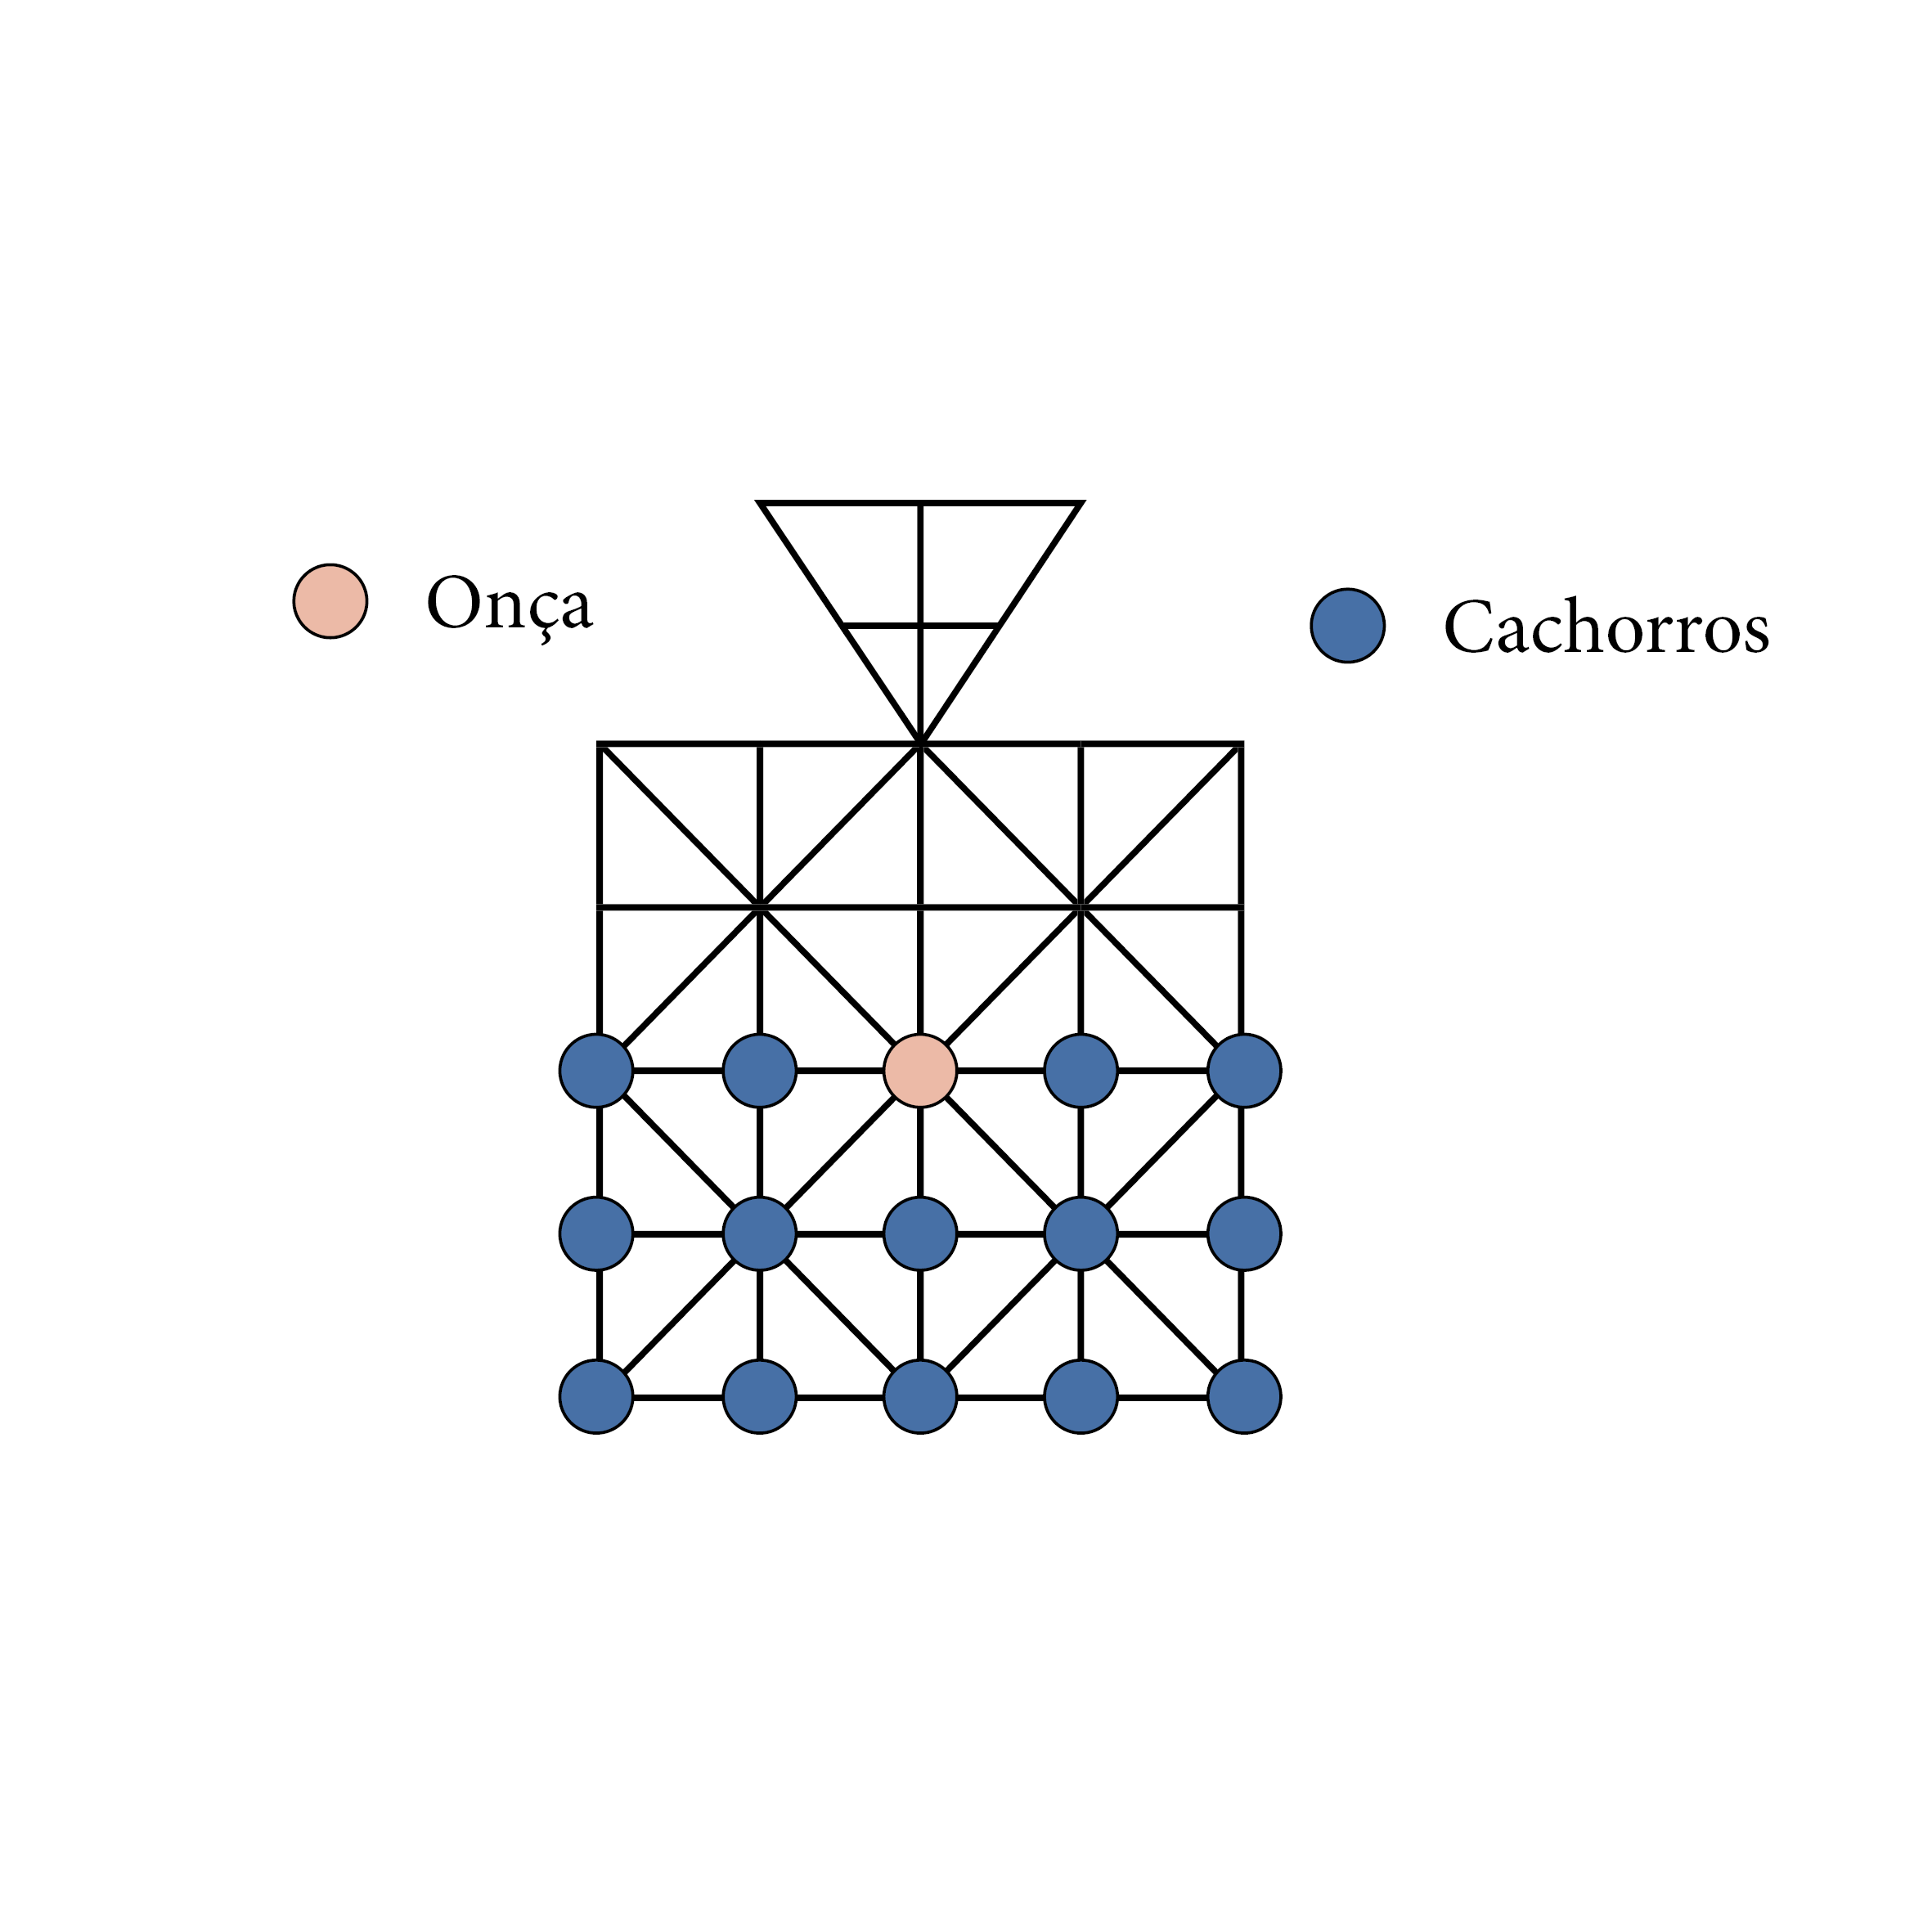
\includegraphics[width=\textwidth]{../ilustracoes/ART5/SAEB_5ANO_ART_FIGURA16.png}
\end{figure}

Um dos cachorros é quem dá início à partida. Tanto os cães como a onça
podem andar para uma casa vizinha vazia por vez, em qualquer direção. A
onça tentará capturar cinco cachorros da mesma forma que ocorre em um
jogo de dama, ou seja, pulando o cachorro e se dirigindo à próxima casa
vazia. Como ocorre no jogo de damas também, é permitido capturar os
cães em sequência. Já os cachorros não podem capturar a onça, ou melhor,
não podem eliminar sua peça representativa do jogo, mas sim cercá-la por
todos os lados. Dessa maneira, a onça ficará imobilizada e os cachorros
vencem a partida. A onça vence quando capturar seis cachorros.

% \coment{Após a leitura do texto sobre o jogo da onça, assista com
% os alunos a este dois vídeos: \emph{Jogo da Onça – Tabuleiro do Suetônio}, disponível em:
%   \emph{https://www.youtube.com/watch?v=VQwCfAGJt-M}; \emph{Jogo da onça – aprenda a jogar},
%   disponível em: \emph{https://www.youtube.com/watch?v=yE1oDk1-m2E}. Acessos em: 22 mar. 2023.
%   No primeiro vídeo, é explicada a confecção do tabuleiro, além de se apresentar a movimentação
%   das peças e os objetivos do jogo. No segund vídeo, apresentam-se algumas estratégias do jogo.
%   Depois, ajude-os a confeccionar o tabuleiro e a definir as peças (bolinhas de papel ou massinha,
%   tampinhas, pedras etc.). Finalmente, forme duplas para que os alunos possam jogar.}

\bigskip
\bigskip
\num{7}  Sobre a literatura de cordel, responda aos itens a seguir.

\begin{escolha}
\item O que é a literatura de cordel?\\
\reduline{Trata-se de uma manifestação artística que combina escrita, oralidade e gravura.\hfill}
\linhas{1}

\item Qual é a origem da literatura de cordel?\\
\reduline{A literatura de cordel é de matriz portuguesa.\hfill}
\linhas{2}

\item O que é a xilogravura?\\
\reduline{Trata-se de uma gravura a partir do entalhe de uma matriz de madeira, que recebe uma fina camada de tinta e depois é “carimbada” no papel, com o que o desenho é transferido para o papel.\hfill}

\item Quais são as características principais da xilogravura?\\
\reduline{A xilogravura conta com grandes contrastas, uso intenso da cor preta e formas simplificadas.\hfill}
\linhas{2}
\end{escolha}

% \coment{Após a realização da atividade,
% assista com os alunos ao vídeo \emph{Xilogravura em isopor
% (isogravura) – tinta preta}, disponível em:
% \emph{https://www.youtube.com/watch?v=YTppa6VsuFM} (acesso em: 22 mar.
% 2023). Assim, os alunos relembram como fazer e criar xilogravuras por
% meio da técnica “isogravura” (xilogravura com isopor). Para criar as
% xilogravuras, serão necessários os seguintes materiais:
% tinta preta, lápis, caneta, bandeja de isopor e papel sulfite.
% A seguir, ajude-os a confeccionar uma xilogravura com tema livre.
% As xilogravuras criadas podem ser expostas na escola para a comunidade apreciar.}

\pagebreak
\num{8}  Observe a imagem a seguir.

\begin{figure}[htpb!]
\centering
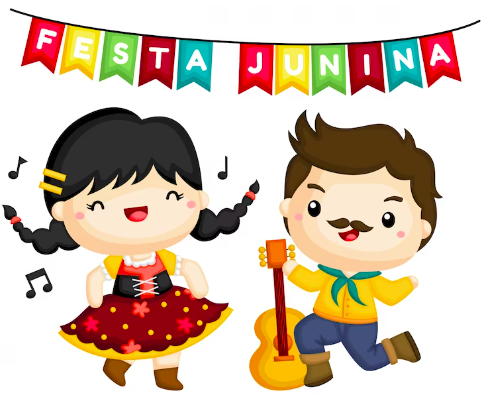
\includegraphics[width=\textwidth]{./imgs/art42.png}
\end{figure}

\noindent{}Sobre a festa a que essa imagem remete, responda quais são as matrizes estéticas e culturais da Festa de São João?

\reduline{As matrizes da Festa de São João são: portuguesa, africana e indígena.\hfill}
\linhas{3}


\num{9} Leia o texto.

\begin{myquote}
\textbf{Conheça o artesanato quilombola}\\
\textit{Baseada em conhecimentos ancestrais dos negros africanos escravizados no Brasil, essa atividade permanece como símbolo identitário.}

{[}\ldots{}{]}

Nascido do trabalho dos negros que buscavam a liberdade fugindo das
senzalas, o artesanato quilombola se destaca pelo uso de vários recursos
naturais para a confecção de objetos e instrumentos de trabalho. Alguns
desses materiais são a madeira, a taquara, a palha de milho, a fibra de
bananeira, a canela e a piaçava. Esse artesanato é, então, o resultado
de um rico repertório de bens culturais que expressam os modos
quilombolas de fazer, sentir e se relacionar com a natureza e com a
própria comunidade.

É um trabalho que preserva e promove tanto as técnicas ancestrais quanto
as matérias-primas naturais, disponíveis no ambiente onde vivem e
interagem. Embora o artesanato quilombola tenha se constituído em uma
importante fonte de renda para essas comunidades, a produção artesanal
para a comercialização não é o único fim dessa atividade.

Na vida quilombola, o artesanato tem inúmeras finalidades funcionais,
como a fabricação de utensílios, vestuário e ornamentos para domicílios.
Muitas atividades ajudam na preservação ambiental, como o artesanato com
palha de bananeira ou o de piaçava, usado para fazer vassouras.

Mas o artesanato quilombola também tem propósitos ritualísticos, de
resgate da memória e da cultura histórica das comunidades negras, para
que as gerações mais jovens se reconheçam no coletivo onde estão
inseridas.

{[}\ldots{}{]}

\fonte{SEBRAE. Conheça o artesanato quilombola. Disponível em:
\emph{https://www.sebrae.com.br/sites/PortalSebrae/artigos/conheca-o-artesanato-quilombola,0c3a17f4bd962810VgnVCM100000d701210aRCRD}.
Acesso em: 22 mar. 2023.}
\end{myquote}

Com base no texto, responda aos itens a seguir.

\begin{escolha}
\item Como o artesanato quilombola é uma expressão da comunidade?\\
\reduline{É um modo de fazer, sentir e se relacionar com a natureza e com a própria comunidade.\hfill}

\item Quais são os recursos naturais utilizados no artesanato quilombola?\\
\reduline{São estes: madeira, taquara, palha de milho, fibra de bananeira, canela e piaçava.\hfill}

\item Qual é a finalidade funcional do artesanato quilombola?\\
\reduline{Utensílios, vestuário, ornamentos para domicílios.\hfill}

\item Que outras finalidades tem o artesanato quilombola?\\
\reduline{Rituais e resgate da memória e da cultura histórica das comunidades negras.\hfill}
\end{escolha}

\num{10} Leia o texto.

\begin{figure}[htpb!]
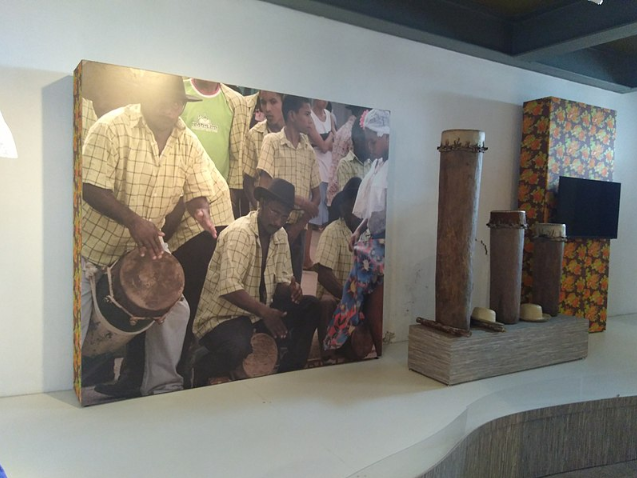
\includegraphics[width=\textwidth]{./imgs/art29.png}
\caption{Instrumentos utilizados no Tambor de Crioula: tambor grande, meião e crivador.}
%\emph{https://commons.wikimedia.org/wiki/File:Casa_do_Tambor_de_Crioula_-_06.jpg}
\end{figure}

\begin{myquote}
{[}\ldots{}{]} ocorre na maioria dos municípios do
Maranhão, envolvendo uma dança circular feminina, canto e percussão de
tambores. Dela participam as coreiras ou dançadeiras, conduzidas pelo
ritmo intenso dos tambores e pelo influxo das toadas evocadas por
tocadores e cantadores, culminando na punga ou umbigada – gesto
característico, entendido como saudação e convite.

\fonte{Felipe Santos. Palmares Fundação Cultural. Tambor de Crioula do Maranhão Patrimônio Cultural Imaterial Brasileiro. Disponpivel em: \emph{https://www.palmares.gov.br/?p=37269}. Acesso em: 22 mar. 2023.}
\end{myquote}

Defina o patrimônio imaterial Tambor de Crioula do Maranhão.

\reduline{É uma forma de expressão de matriz afro-brasileira que envolve dança
circular, canto e percussão de tambores. É realizado sem local
específico ou calendário pré-fixado.\hfill}
%\linhas{3}

\section*{Treino}

\num{1}  Nas terríveis viagens da África para o Brasil, as mães escravizadas
rasgavam retalhos de suas saias e, com eles, criavam pequenas bonecas, feitas
de tranças ou nós, e usavam para acalentar seus filhos, além de usá-las como
amuleto de proteção. Símbolo de resistência, as bonecas ficaram conhecidas
como \textbf{abayomi}. O termo tem origem no iorubá e significa algo como
“encontro precioso”.

Assinale a alternativa que contém uma imagem de boneca abayomi.

%\begin{minipage}{.8\textwidth}
%\acima{\hspace*{-8cm} a) \hspace{4cm} b)}
%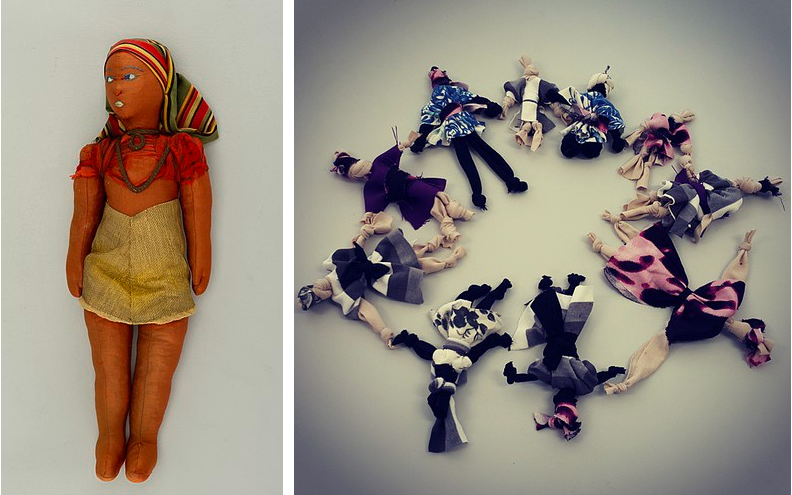
\includegraphics[width=\textwidth]{./imgs/art30ab.png}
%
%\acima{\hspace*{-8cm} c) \hspace{4cm} d)}
%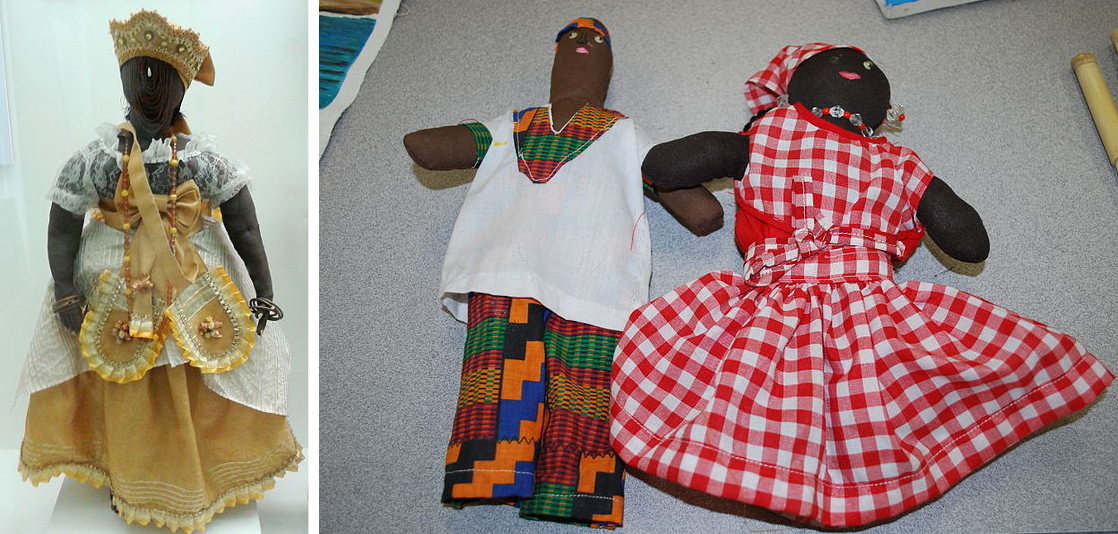
\includegraphics[width=\textwidth]{./imgs/art30cd.png}
%\end{minipage}\hspace{.5cm}
%\begin{minipage}{.2\textwidth}
%\end{minipage}\pagebreak

\begin{figure}[htpb!]
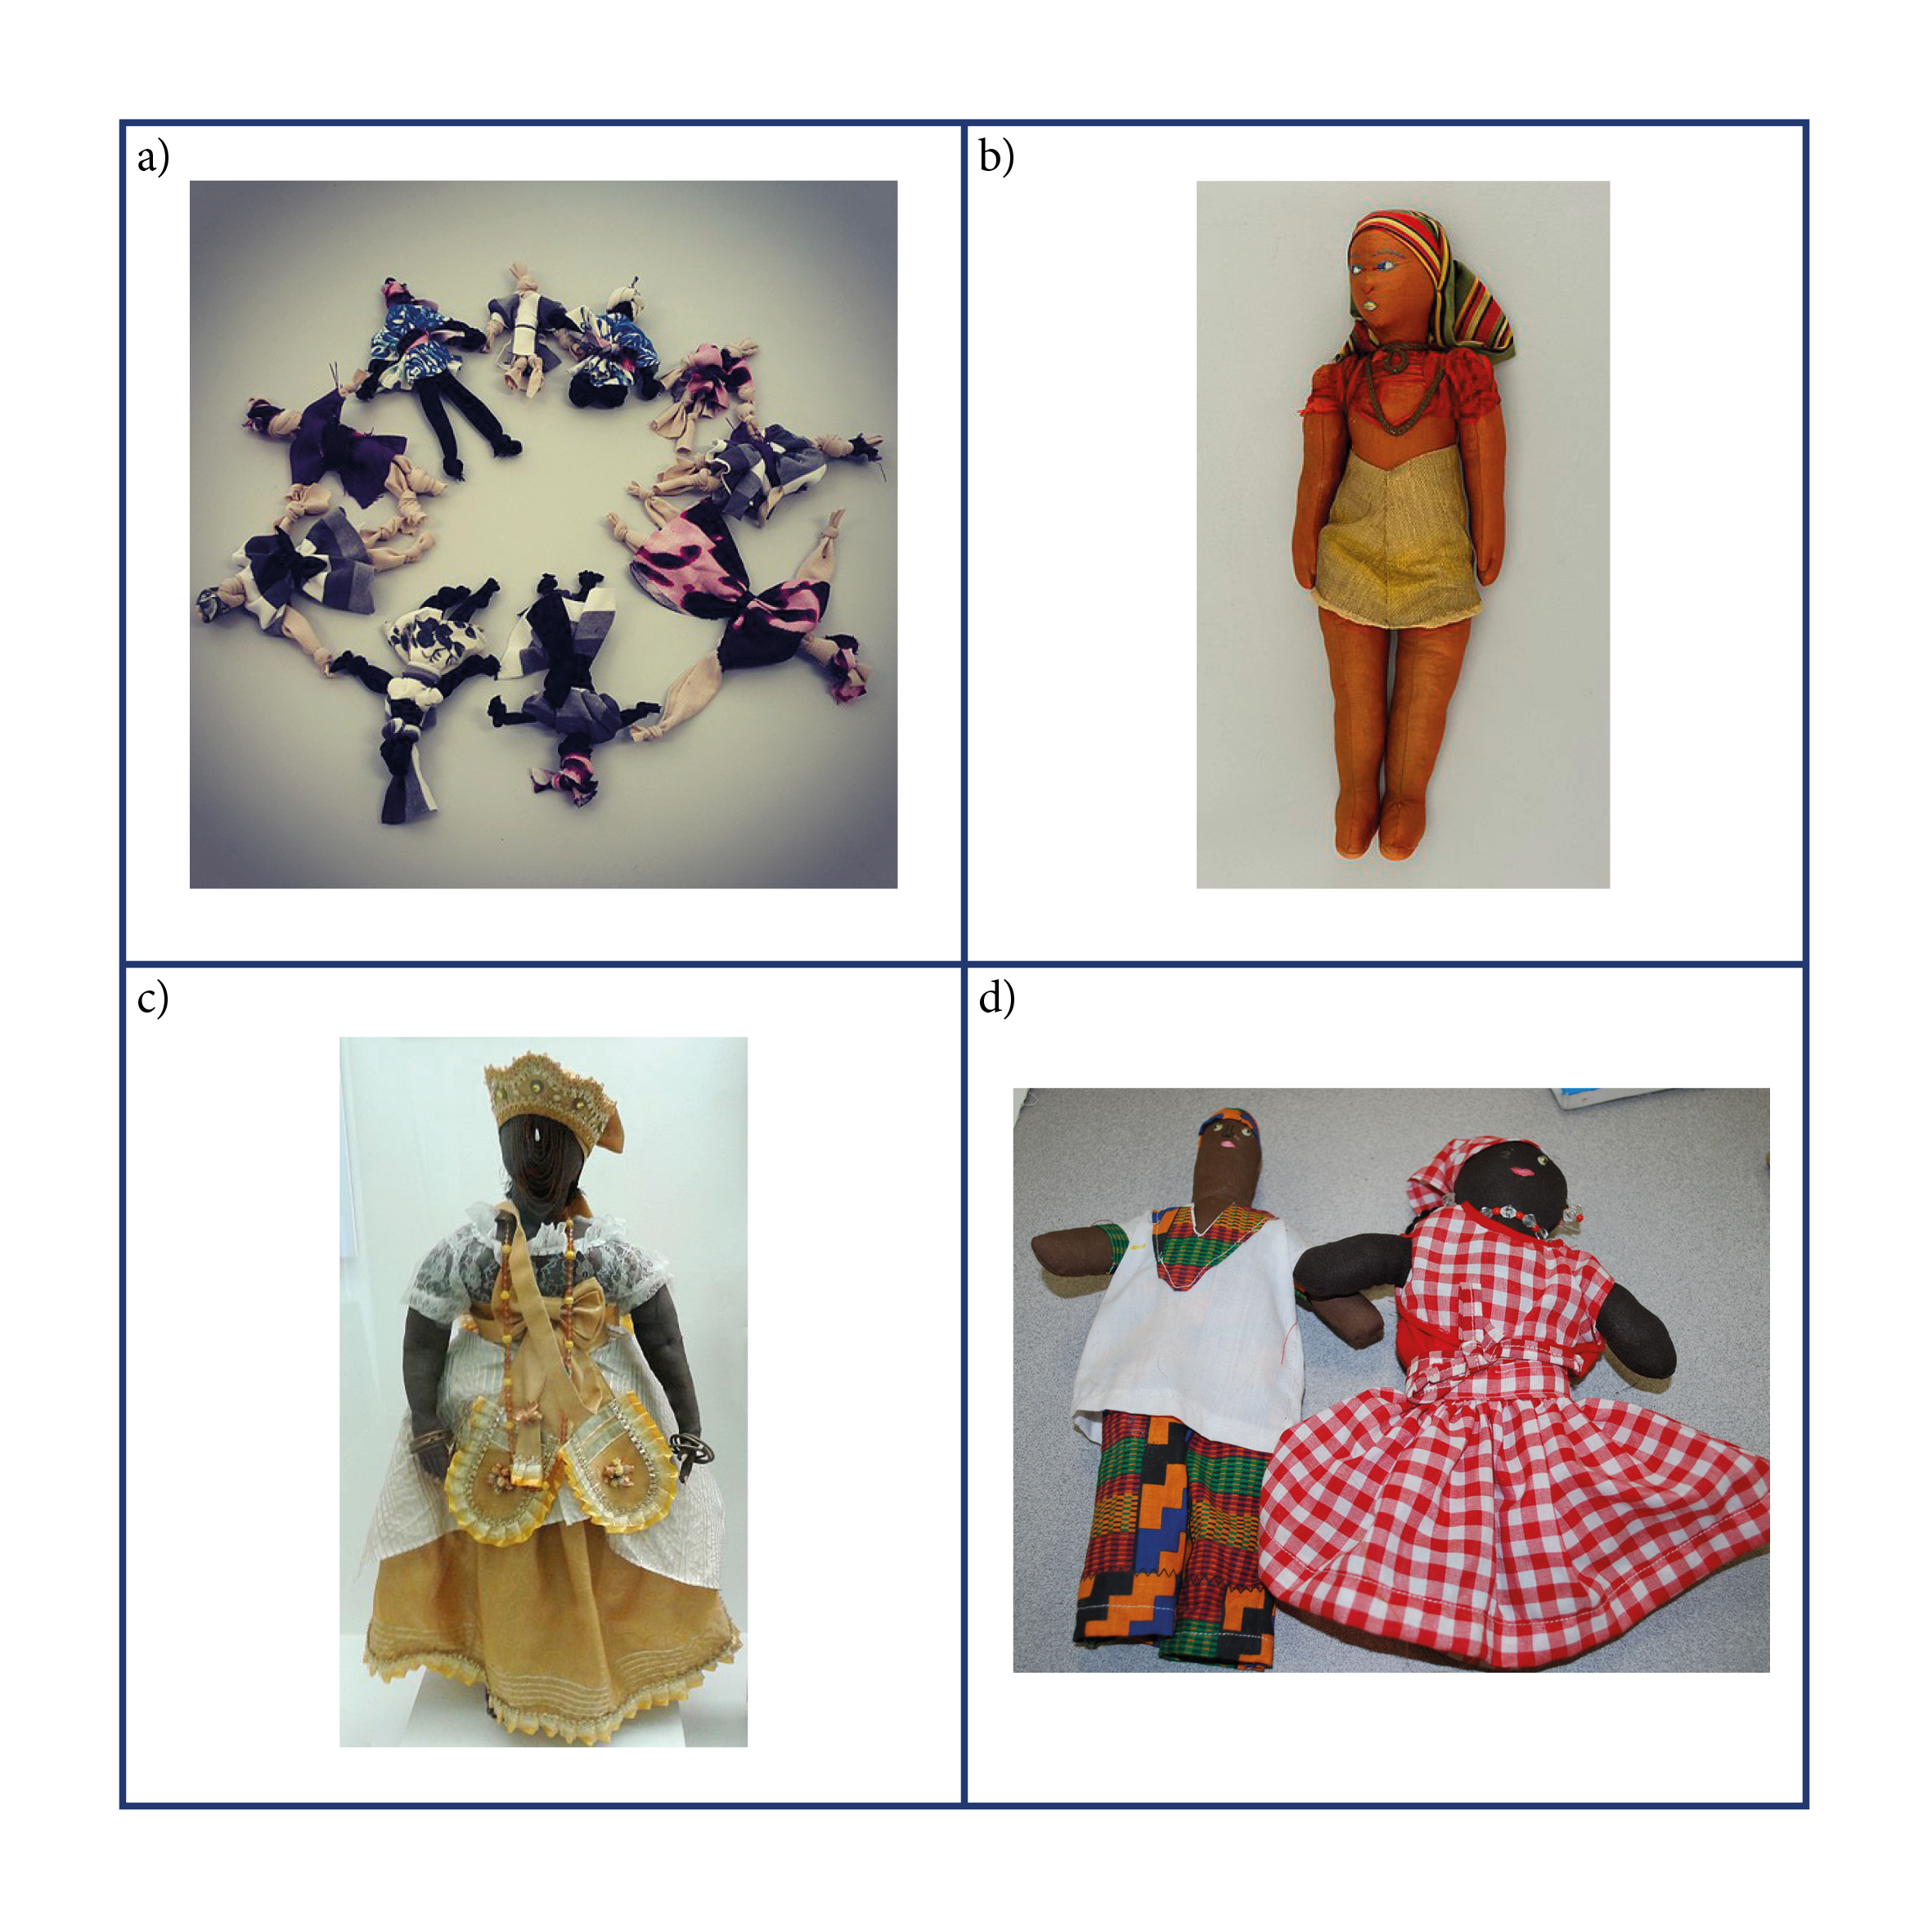
\includegraphics[width=\textwidth]{../ilustracoes/ART5/SAEB_5ANO_ART_FIGURA19.png}
\end{figure}



\num{2}  Assinale a alternativa que contém a descrição de um patrimônio imaterial.

\begin{escolha}
\item
  A cidade de Ouro Preto e a primeira cidade brasileira a receber o
  título de Patrimônio Mundial, conferido pela Unesco, em 1980. Seu
  traçado urbano colonial mantém-se intacto e o mesmo ocorre com os
  exemplares da arquitetura religiosa e civil, e as suas obras de arte
  preservadas.
\item
  O Parque Estadual Veredas do Peruaçu, situado no município de Cônego
  Marinho (MG), abriga um complexo de veredas e lagoas, dentre as quais
  está a vereda do Peruaçu (que significa gruta grande) que dá nome ao
  parque.
\item
  Os mestres de capoeira são detentores dos conhecimentos tradicionais
  da manifestação Roda de Capoeira e responsáveis pela transmissão de
  suas práticas, rituais e herança cultural.
\item
  A Igreja Matriz de Nossa Senhora da Conceição, construção do século
  XVIII, destaca-se pelo suporte arquitetônico e por seu interior. O
  frontispício, com seu belo pórtico esculpido, é obra do Aleijadinho.
\end{escolha}


\num{3}  Observe a imagem.

\begin{figure}[htpb!]
\centering
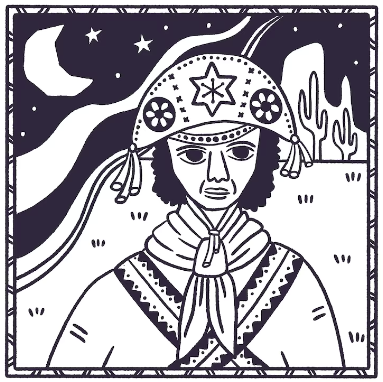
\includegraphics[width=.5\textwidth]{./imgs/art43.png}
\end{figure}

Essa imagem relaciona-se a um patrimônio cultural brasileiro. Sobre o assunto, assinale uma alternativa que descreve corretamente esse patrimônio.

\begin{escolha}
\item
  Gênero literário em prosa.
\item
  Temas populares da cultura africana.
\item
  Literatura de tradição regional.
\item
  Linguagem culta (formal).
\end{escolha}



